%=======================================================================
%  ARTICLE II
%  A Doubly Slotted Annulus Operator for Magnetic Equivalent Circuits:
%  Carter's Factor Is Low in the Thin-Gap, Wide-Opening Regime, on an
%  18.5 kW Cage Induction Machine
%
%  TITRE CHANGE (revue, C-2) : l'ancien titre -- « A +5 % Correction to
%  Carter's Factor » -- affirmait une valeur ponctuelle que la Table 2
%  du present manuscrit montre non convergee (dispersion 6,82 % sur neuf
%  pavages, contre une correction annoncee de 5,2 %). Le resultat que les
%  donnees soutiennent est un ENCADREMENT, non un point.
%
%  Gabarit NEUTRE (SPEC_CLAUDE_CODE_v3 §9), identique a l'Article I.
%
%  ETAT : sections 3, 4 et 6 redigees (le coeur) ; 1, 2, 5, 7 en
%  squelette avec leur provenance ; 8 a ecrire en dernier.
%
%  Cree le 5 aout 2026 ; reconstruit et etoffe le 6 aout 2026.
%=======================================================================
\documentclass[10pt,a4paper,twocolumn]{article}

\usepackage[T1]{fontenc}
\usepackage[utf8]{inputenc}
\usepackage{mathptmx}                 % Times-like serif body
% Times pour tout le document : titres compris (pas de sans-serif)
\usepackage[left=20mm,right=20mm,top=24mm,bottom=24mm,
            columnsep=7mm]{geometry}
\usepackage{amsmath,amssymb,bm}
\usepackage{siunitx}
\usepackage{graphicx}
\usepackage{booktabs,threeparttable}
\usepackage[font=small,labelfont=bf,labelsep=period,
            justification=centering]{caption}
\usepackage{enumitem}
\usepackage{stfloats}
\usepackage{flafter}
\setcounter{topnumber}{3}
\setcounter{bottomnumber}{2}
\setcounter{totalnumber}{4}
\setcounter{dbltopnumber}{2}
\renewcommand{\topfraction}{0.92}
\renewcommand{\bottomfraction}{0.6}
\renewcommand{\floatpagefraction}{0.88}
\usepackage[hidelinks]{hyperref}
\usepackage[numbers,sort&compress]{natbib}
\usepackage{doi}          % prints the DOI of every reference that has one
\usepackage[explicit]{titlesec}

\titleformat{\section}{\rmfamily\bfseries\fontsize{11.5}{14}\selectfont}{\thesection.}{0.7em}{#1}
\titleformat{\subsection}{\rmfamily\bfseries\fontsize{10.5}{12.5}\selectfont}{\thesubsection.}{0.6em}{#1}
\titleformat{\subsubsection}{\rmfamily\itshape\fontsize{9.5}{11.5}\selectfont}{\thesubsubsection.}{0.5em}{#1}
\titlespacing*{\section}{0pt}{11pt plus 3pt minus 2pt}{5pt plus 1pt}
\titlespacing*{\subsection}{0pt}{8pt plus 2pt minus 1pt}{3pt plus 1pt}
\titlespacing*{\subsubsection}{0pt}{7pt plus 2pt minus 1pt}{2.5pt}
% Le point final est porte par le titre et non par le compteur : sans cela
% \ref produit << Section 5.2.. >> en fin de phrase.
\renewcommand{\thesection}{\arabic{section}}
\renewcommand{\thesubsection}{\arabic{section}.\arabic{subsection}}
\renewcommand{\thesubsubsection}%
  {\arabic{section}.\arabic{subsection}.\arabic{subsubsection}}
\setlength{\abovecaptionskip}{4pt}
\setlength{\belowcaptionskip}{2pt}
\setlength{\parindent}{0pt}
\setlength{\abovedisplayskip}{5.5pt plus 1.5pt minus 1pt}
\setlength{\belowdisplayskip}{5.5pt plus 1.5pt minus 1pt}
\setlength{\abovedisplayshortskip}{3pt plus 1pt}
\setlength{\belowdisplayshortskip}{3.5pt plus 1pt}
\setlength{\jot}{3pt}
\setlength{\parskip}{3.2pt plus 1pt minus 0.5pt}
\setlength{\textfloatsep}{9pt plus 2pt minus 2pt}
\setlength{\intextsep}{8pt plus 2pt minus 2pt}
\setlength{\floatsep}{7pt plus 2pt minus 2pt}
\setlength{\dbltextfloatsep}{10pt plus 2pt minus 2pt}
\renewcommand{\dbltopfraction}{0.92}
\renewcommand{\dblfloatpagefraction}{0.92}
\renewcommand{\textfraction}{0.10}

\graphicspath{{figures/}}

\DeclareSIUnit{\ampereturn}{At}
\DeclareSIUnit{\rpm}{rpm}
\DeclareSIUnit{\pp}{p.p.}
% \textohm is absent from the T1 Times text companion and prints as a
% black box; the math glyph is used instead. Rendering only, no unit change.
\DeclareSIUnit{\ohm}{\ensuremath{\Omega}}
\sisetup{detect-all,per-mode=symbol,range-phrase={--},range-units=single}

\newcommand{\Rs}{R_{\mathrm{s}}}
\newcommand{\Rro}{R_{\mathrm{ro}}}
\newcommand{\rmi}{r_{\mathrm{mi}}}
\newcommand{\murec}{\mu_{\mathrm{r}}}
\newcommand{\Ua}{U_{\mathrm{a}}}
\newcommand{\Um}{U_{\mathrm{m}}}
\newcommand{\Xg}{X_{\mathrm{g}}}
\newcommand{\keywordsline}[1]{\par\noindent\textbf{Keywords}\quad #1}

\usepackage{amsthm}
\theoremstyle{plain}
\newtheorem{proposition}{Proposition}
% Le carre de fin de demonstration (halmos) est retire a la demande de l'auteur.
\renewcommand{\qedsymbol}{}
\theoremstyle{remark}
\newtheorem{remark}{Remark}

\begin{document}

\twocolumn[
\begin{center}
{\rmfamily\bfseries\fontsize{15}{19}\selectfont
A Doubly Slotted Annulus Operator for Magnetic Equivalent
Circuits: Carter's Factor Is Low in the Thin-Gap, Wide-Opening Regime,
on an \SI{18.5}{\kilo\watt} Cage Induction Machine\par}
\vspace{7mm}
{\rmfamily\bfseries\fontsize{10}{13}\selectfont
Idris Laouar$^{1}$ $\cdot$ Ahcene Boukadoum$^{1}$ $\cdot$ Nabil Mezhoud$^{1}$\par}
\end{center}
\vspace{6mm}

{\rmfamily\bfseries Abstract}\par\vspace{2pt}
A magnetic equivalent circuit closes its air gap with an empirical permeance
function, on a cage induction machine, Carter's factor, derived for a
\emph{single, isolated} slot in an infinite half-plane. We replace it by the
exact Dirichlet-to-Neumann operator of an annulus bounded by \emph{two}
slotted surfaces, tiled exactly by tooth faces and openings, eliminating
the opening unknowns by a Schur complement onto the tooth nodes. The
redistribution beneath the opening is solved, not modelled; no fringing
coefficient, effective gap or coupling width enters. Condensed in a
conforming surface basis the operator has a limit, and the slotting ratio
exceeds the classical value at all nine tilings by
\SI{2.5}{\percent} to \SI{9.7}{\percent}. \emph{That the classical value is
low in this regime is established; by how much is not}: bounding the
excess, at an opening \num{8.23} times the gap with both surfaces
slotted, is the contribution, and no corrected value is proposed. Every
reported value is a lower bound in two measured senses: the tiling has not
converged, and the finite iron reluctance in both solves compresses the
ratio towards unity, its removal raising it by \SI{20.3}{\percent}. Against
finite elements on an \SI{18.5}{\kilo\watt} machine, rated torque agrees
within \SI{6.0}{\percent} and stator current within \SI{3.2}{\percent}, but the
magnetising current is high by \SI{21.6}{\percent}: the error
is displaced, not removed. The case for the converged closure is existence,
not accuracy: a number that changes with the truncation is not a prediction,
even when it falls closer to the reference.
\vspace{4mm}

{\rmfamily\bfseries Keywords}\quad Magnetic equivalent circuit $\cdot$ Reluctance network
$\cdot$ Dirichlet-to-Neumann operator $\cdot$ Doubly slotted air gap
$\cdot$ Carter's factor $\cdot$ Schur complement $\cdot$ Cage induction
machine $\cdot$ Finite-element validation
\vspace{4mm}
\vspace{5mm}

\begin{center}{\rmfamily\bfseries Nomenclature}\end{center}
\vspace{-1mm}
{\footnotesize
\parbox[t]{0.485\textwidth}{\begin{tabular}{@{}p{16mm}p{56mm}@{}}
$\varphi$ & magnetic scalar potential (A)\\
$u_{\mathrm{s}}$, $u_{\mathrm{r}}$ & bore potential, stator / rotor side\\
$\Rs$, $\Rro$ & stator bore and rotor outer radius\\
$\Xg$ & logarithmic thickness of the air annulus\\
$g$, $b_0$, $L$ & air gap, slot opening, active length\\
$B_r$, $B_t$ & radial and tangential flux density\\
$p$, $N_{\mathrm{s}}$, $N_{\mathrm{r}}$ & pole pairs, stator and rotor slots\\
$\nu$, $n$ & spatial order of an air-gap harmonic\\
$s$ & slip\\
$\Lambda_0$ & homopolar permeance\\
\end{tabular}}\hfill
\parbox[t]{0.485\textwidth}{\begin{tabular}{@{}p{16mm}p{56mm}@{}}
$\bm{Y}$ & condensed bore admittance matrix\\
$W_n$ & projection of the basis onto order $n$\\
$H^{1/2}$ & trace space of the annulus problem\\
$N_h$ & harmonic truncation\\
$n_T$, $n_O$ & tiling columns per tooth face / slot opening\\
$k_{\mathrm{C}}$ & Carter's slotting ratio\\
$X_m$, $X_{m0}$ & magnetising reactance, saturated and unsaturated\\
$I_0$, $E_1$ & no-load current, air-gap electromotive force\\
$R_s$, $R'_r$ & stator and referred rotor resistance\\
$X_{\sigma s}$, $X_{\sigma r}$ & stator and rotor leakage reactance\\
$\delta$ & skin depth in a rotor bar\\
\end{tabular}}\par}

]

\footnotetext[1]{Department of Electrical Engineering, Electrotechnical
Laboratory Skikda (LES), University 20 August 1955, 26 Road El Hadaiek,
21000 Skikda, Algeria. Corresponding author: Idris Laouar,
\texttt{idris.laouar@univ-skikda.dz}.}
%=======================================================================
\vspace{4mm}

\clearpage
%=======================================================================
\section{Introduction}
\label{sec:intro}

\subsection{A Network Element Not Derived from the Geometry}

A magnetic equivalent circuit represents a machine by lumped branches
carrying the true $B(H)$ characteristic, so that saturation is captured
natively and arbitrary slot shapes remain admissible at a cost far below
that of finite elements. For cage induction machines the formulation is
mature~\cite{ostovic1989,ostovic1986,perho2002,hosseini2026}.

Its economy is paid at one place, and always the same. A branch is
defined by a path through iron whose length and cross-section the
geometry supplies; the annulus separating the two iron surfaces has no
such path, and projecting its continuous field onto a finite number of
tooth-to-tooth tubes requires a permeance the network cannot furnish
from its own construction. Every element of a magnetic equivalent
circuit is therefore obtained from geometry and material data except
one, and that one governs the accuracy of all the others. On a cage
induction machine it is supplied by Carter's factor~\cite{carter}.

\subsection{Propagation of the Air-Gap Coefficient Through the Model}

The reach of $k_{\mathrm{C}}$ is easily understated, because it enters
as a single scalar and leaves as a design point. Replacing the slotted
geometry by a smooth one with gap $g_{\mathrm{eff}}=k_{\mathrm{C}}g$
sets the magnetising reactance directly; that reactance sets the no-load
current, hence the power factor and the light-load copper loss, and the
tooth saturation level, hence the iron loss; and through the equivalent
circuit it enters the torque and the rated slip. The coefficient
propagates to every quantity a designer specifies, and it does so
without an error bar, because none has been established: a designer
using $k_{\mathrm{C}}$ cannot tell, from within the method, how far the
answer lies from the field solution it approximates.

The magnitude of that propagation is not hypothetical. The closure
Carter's factor supplies normalises the tooth permeances so that their
sum reproduces $\mu_0 L\tau_{\mathrm{s}}/(k_{\mathrm{C}}g)$ exactly;
removing that normalisation and solving the annulus instead moves the
computed no-load current of this machine from \SI{+1.5}{\percent} to
\SI{+21.6}{\percent} relative to the finite-element reference. The
agreement the classical closure displays on that quantity is therefore
not a prediction: it is the normalisation, read back. For that branch of
the circuit the construction is not a correction applied to a solved
problem, it is the solution.

Nor is the regime in which the classical hypotheses fail an unusual
one. The two quantities whose ratio decides the matter are set by
opposing constraints that every cage design must reconcile. The
mechanical gap is made as small as bearing tolerance and rotor dynamics
permit, because the magnetising current varies inversely with it and
the power factor follows; the slot opening, by contrast, cannot fall
below the width required to insert the conductors and retain the wedge,
and it is bounded below by manufacturing rather than by
electromagnetics. The two are therefore pushed apart by design, not
brought together, and a ratio of several units is the normal outcome
instead of an extreme case: the machine studied here has
$b_0/g=\num{8.23}$. Whatever error the isolated-slot assumption carries
in that regime is thus incurred routinely, and by a population of
machines that the single-slot hypothesis was never derived to
cover.

\subsection{Failure of the Classical Hypotheses and Limitations of Existing Alternatives}

Carter's construction maps a \emph{single, isolated} slot in an infinite
half-plane by conformal transformation~\cite{carter,pyrhonen}. Two of
its hypotheses fail together here, and they fail in the regime where
induction machines are designed. The slot opening is not small compared
with the gap, $b_0/g=\num{8.23}$, so neighbouring slots interact
through the gap rather than each perturbing an otherwise uniform field;
and \emph{both} surfaces are slotted, whereas the classical treatment
corrects one surface at a time and multiplies the two factors. Thin gaps
and wide openings are not exotic: they are what a cage induction machine
has.

The alternatives each remove one limitation while keeping another.
Complex relative permeance functions give both field components but are
exact only for a slotted stator facing a \emph{smooth}
rotor~\cite{zarko2006b}. Subdomain methods solve the slotted geometry
exactly~\cite{lubin2010} but assume infinitely permeable iron, which is
the phenomenon a magnetic equivalent circuit exists to capture.
Parametric tooth-to-tooth permeance functions keep the network and the
saturable iron, but tie the permeance to the discretisation of the two
surfaces rather than to the geometry~\cite{silva2023}. Nearest of all
is the air-gap element, codified in textbook form by
Salon~\cite{salon1995} and generalised to a wide class of geometries by
the harmonic transfer-relation formulation of Gysen \emph{et
al.}~\cite{gysen2010}, together with its descendants, which expand the
annulus in
harmonics and attach it either to a finite-element
domain~\cite{abdelrazek1982,degersem2004} or, in the hybrid
formulations, to a reluctance network~\cite{ouagued2016,belmahi2026};
none of them returns a
slotting ratio for a doubly slotted annulus with saturable iron and no
fitted quantity.

\subsection{Research Gap and the Reasons for Its Persistence}

\emph{The gap is narrower than a blanket claim of novelty, and stating it
narrowly is what makes it defensible.} Carter's accuracy has been
assessed before, and Section~\ref{sub:priorwork} discusses three such
studies~\cite{viorel2007,viorel2014,sharifian2003}. What those studies
share, and what leaves the present question open, is twofold: the
reference is a finite-element \emph{field} from which a factor is
\emph{inferred} by a chosen definition, and the corrected geometry has
\emph{one} slotted surface. \emph{A directly computed slotting ratio,
for a doubly slotted annulus, obtained without inferring it from a field,
is what is missing}, and it is what the operator of
Section~\ref{sec:twosurface} returns of its own accord. Nothing cheaper has been available for
the doubly slotted case, so the assumption has been carried forward for
want of an alternative; and the natural arbiter, a finite-element
solution of the same annulus, answers a different question, since it
returns a field and not a ratio. Obtaining the ratio requires solving
the smooth and the slotted geometry under otherwise identical
conditions, a controlled substitution rather than a computation.

An exactly condensed annulus operator makes that substitution available:
removing the slotting and re-solving yields the two reactances whose
ratio \emph{is} the slotting factor, measured on the solution rather
than imposed on it. One condition attaches, and it is not a formality.
Such a ratio is a property of the geometry only if the condensation
converges, and Appendix~\ref{app:trace} shows that under the
piecewise-constant surface basis that a reluctance network naturally
uses, the series diverges, so a ratio read off it would be a property
of the harmonic count and not of the annulus. Section~\ref{sec:p1}
therefore verifies the condition before Section~\ref{sec:carter} uses
it.

\subsection{Aim and Contributions}

This paper derives the Dirichlet-to-Neumann operator of an annulus
bounded by two slotted iron surfaces, condenses it onto the tooth nodes
of a saturable reluctance network without any fitted air-gap quantity,
and uses it to measure the slotting ratio of an \SI{18.5}{\kilo\watt}
cage induction machine against two-dimensional finite elements.

Three contributions are claimed. The operator itself is condensed
without a fringing parameter: both bores are tiled so that tooth faces
and slot openings pave them exactly, and the opening degrees of freedom
are eliminated by a Schur complement, so the redistribution of flux
beneath the opening is solved rather than modelled
(Section~\ref{sec:twosurface}). The error of Carter's factor is
\emph{bounded}: over nine tilings the converged-basis ratio exceeds the
classical value at every point, by between \SI{2.5}{\percent} and
\SI{9.7}{\percent}, with no fitted coefficient anywhere in the
chain: the excess is expected in this regime, and what is new is that
it is measured against a solution making none of Carter's assumptions
(Section~\ref{sec:carter}). No single corrected value is proposed,
because the tiling axis has not been closed. And the price is stated
instead of absorbed: the no-load current moves to
\SI{+21.6}{\percent} above the reference, the error being concentrated
on the magnetising branch while everything depending on it weakly
improves (Section~\ref{sec:price}).

Because a numerical reference carries its own discretisation error,
Section~\ref{sec:im} states what each reference quantity is and how it
was obtained before any agreement is asserted, a precaution that, in
the course of this work, reversed the sign of one reported deviation.

%======================================================================

\section{The Doubly Slotted Annulus Operator}
\label{sec:twosurface}

\subsection{Two-Surface Formulation of the Annulus Operator}
\label{sub:twosurface}

A single-surface annulus operator assumes the inner boundary to be
infinitely permeable and at zero potential, which is the surface-magnet
geometry. A cage induction machine violates that assumption: both
bounding surfaces are slotted iron carrying an unknown potential. The
operator for that case is not obtained by specialising the preceding
one, removing the magnet layer yields the single-surface air annulus,
not a two-surface map, and is derived here.

Let the annulus be air, $\Rro \le r \le \Rs$ with $\Rro$ the rotor bore,
and write $\Xg=\ln(\Rs/\Rro)$ and $v=\ln(r/\Rro)$. In the absence of
current the scalar potential is harmonic, and in the logarithmic
coordinate $v$ each Fourier order obeys
$\varphi_n''=n^2\varphi_n$. Both surfaces carry a Dirichlet datum,
$u_{\mathrm{s}}$ at $\Rs$ and $u_{\mathrm{r}}$ at $\Rro$, so
\begin{equation}
\varphi_n(v)=\frac{u_{\mathrm{r},n}\sinh\!\big(n(\Xg-v)\big)
+u_{\mathrm{s},n}\sinh(nv)}{\sinh(n\Xg)} .
\label{eq:phi_two}
\end{equation}
Throughout, a bore quantity is expanded as
$f(\theta)=\sum_{n\ge1}\big(f^{\mathrm{c}}_n\cos n\theta
+f^{\mathrm{s}}_n\sin n\theta\big)$ with real coefficients, and
$\bm{u}_n=(u^{\mathrm{c}}_n,u^{\mathrm{s}}_n)$ collects the two
quadrature components of order $n$. The magnetic energy stored in the
annulus follows from \eqref{eq:phi_two} as
\begin{equation}
W_n=\frac{\mu_0\pi n L}{2}\left[
\coth(n\Xg)\Big(\|\bm{u}_{\mathrm{s},n}\|^2+\|\bm{u}_{\mathrm{r},n}\|^2\Big)
-\frac{2\,\langle\bm{u}_{\mathrm{s},n},\bm{u}_{\mathrm{r},n}\rangle}
{\sinh(n\Xg)}\right],
\label{eq:W_two}
\end{equation}
with $\langle\cdot,\cdot\rangle$ the Euclidean product of the two
quadrature pairs and $\|\cdot\|$ its norm.

Both surfaces are discretised. Surface node $k$ spans an arc of width
$\Delta\theta_k$ and holds a potential $U_k$, and a basis function
$\chi_k$ describes how the potential is carried across that arc.
Projecting $\chi_k$ onto the Fourier basis gives rectangular operators
$\bm{W}^{\mathrm{c}}$, $\bm{W}^{\mathrm{s}}$, one pair per surface.
\emph{The choice of $\chi_k$ is not innocent and is the subject of
Section~\ref{sec:p1}}; the assembly below holds for any admissible
choice.

Differentiating \eqref{eq:W_two} with respect to the nodal potentials
and projecting gives a block map between the two sets of surface
potentials and the two sets of surface fluxes,
\begin{equation}
\begin{aligned}
\begin{bmatrix}\bm{\Phi}_{\mathrm{s}}\\[2pt]\bm{\Phi}_{\mathrm{r}}\end{bmatrix}
&=\Bigl(\bm{Y}_{\mathrm{h}}+\Lambda_0\,\bm{w}\bm{w}^{\!\top}\Bigr)
\begin{bmatrix}\bm{U}_{\mathrm{s}}\\[2pt]\bm{U}_{\mathrm{r}}\end{bmatrix},\\[4pt]
\bm{Y}_{\mathrm{h}}&=\begin{bmatrix}
\bm{Y}_{\mathrm{ss}} & \bm{Y}_{\mathrm{sr}}\\[2pt]
\bm{Y}_{\mathrm{sr}}^{\!\top} & \bm{Y}_{\mathrm{rr}}\end{bmatrix},
\qquad
\bm{w}=\begin{bmatrix}\bm{w}_{0\mathrm{s}}\\[2pt]-\bm{w}_{0\mathrm{r}}\end{bmatrix},
\end{aligned}
\label{eq:Y_two}
\end{equation}
with $\bm{w}_{0\mathrm{s}}$ and $\bm{w}_{0\mathrm{r}}$ the segment
widths normalised by $2\pi$. The diagonal blocks are built on the kernel
$-\mu_0\pi L\,n\coth(n\Xg)$ and the off-diagonal block on
$+\mu_0\pi L\,n/\sinh(n\Xg)$; the signs are those that make the
assembled operator negative semi-definite. The homopolar permeance is
\begin{equation}
\Lambda_0=\frac{2\pi\mu_0 L}{\Xg} .
\label{eq:Lam0}
\end{equation}

Four remarks complete the picture, each with a counterpart later in the
paper.

\paragraph{The $n=0$ mode must be retained.}
The Fourier projection is undefined at $n=0$, and the harmonic sum alone
leaves the two mean potentials uncoupled. The rank-one term in
\eqref{eq:Y_two} restores the homopolar path: a difference between the
mean stator and mean rotor potentials drives a net radial flux of
permeance $\Lambda_0$. Omitting it leaves the block singular on a mode
that carries real flux.

\paragraph{The operator is semi-definite, with one null mode.}
Raising both surfaces together by the same constant drives no flux, so
$\bm{Y}\,[\bm{1};\bm{1}]=\bm{0}$. The gauge is fixed by the iron
network, exactly as in the single-surface case. That identity is exact on
the continuous operator; \emph{the discrete one inherits it only if the
surface basis represents the constant function exactly}, which is a
condition on $\chi_k$ and on the grid jointly rather than on either
alone. Section~\ref{sub:hatdefect} reports a basis and a grid, both used
in this paper, for which it does not hold.

\paragraph{Position invariance is lost.}
$\bm{Y}_{\mathrm{sr}}$ couples the two tooth patterns through their
relative angular position, so the operator must be reassembled at each
rotor position. The cost is modest, the kernels $\coth(n\Xg)$ and
$1/\sinh(n\Xg)$ are position-independent and only the rotor projection
is rebuilt, but the property that makes a full rotor sweep cost one
factorisation, when one surface is smooth, does not survive here.

\paragraph{Two limits check the implementation.}
Energising one surface with the other grounded yields an energy
coefficient $\mu_0\pi R L/(2g)$ per harmonic, that is the smooth-gap
permeance, since $n\coth(n\Xg)\to R/g$ as $\Xg\to0$. Raising both to the
same potential yields an energy that is purely tangential,
$\mu_0\pi n^2 g L/(2R)$, since
$\coth(n\Xg)-1/\sinh(n\Xg)=\tanh(n\Xg/2)\to n\Xg/2$. The second limit is
the zig-zag flux, which a network of radial branches cannot represent at
all. Both are recovered to machine precision.

\subsection{Tiling of the Two Surfaces and Condensation onto the Tooth Nodes}
\label{sub:tiling}

The operator \eqref{eq:Y_two} cannot be built with one degree of freedom
per tooth. Tooth faces do not pave the bore, the slot openings lie
between them, so a projection defined on tooth nodes alone implicitly
imposes zero flux over the openings, which is not the physical
condition. The consequence is not subtle but diagnostic: the slotting
ratio the operator returns then tends to unity as the harmonic order is
refined, and the slot effect disappears altogether.

The construction that removes this is shown in Fig.~\ref{fig:gapop},
whose three panels state the geometry, the defect and the condensation
in that order. Panel~(a) shows the doubly slotted annulus with the
tiling laid on both bores, $n_T$ columns on each tooth face and $n_O$
over each opening, and the flux crossing from a tooth face into a facing
opening: the path the operator has to resolve. Panel~(b) shows what a
treatment without opening degrees of freedom does instead: with no
unknown over the opening, a null potential is imposed there implicitly,
and the slotting ratio it returns collapses towards unity as the
harmonic count rises, from \num{1.053} to \num{1.024} over the sweep
plotted beneath. Panel~(c) shows the assembled operator as a block
matrix in the tooth and opening unknowns, and the Schur complement that
eliminates the opening block, leaving only the tooth-face block that
reaches the reluctance network, drawn to scale, so that the size of
what is condensed away is visible.

Each tooth pitch is tiled by $n_T$ columns spanning the tooth face and
$n_O$ columns spanning the slot opening, on both surfaces, so that the
columns pave the bore exactly. The arcs are the tooth \emph{faces} seen
from the gap, the pitch less the slot opening, not the tooth body
widths used by the internal mesh, and the distinction matters: it is the
face that bounds the annulus. The exact operator is assembled on this
fine grid, where the Laplace solution is exact, and then condensed onto
the tooth nodes of the performance network by two conditions, both
physical and neither fitted:

\begin{figure*}[!tb]
\centering
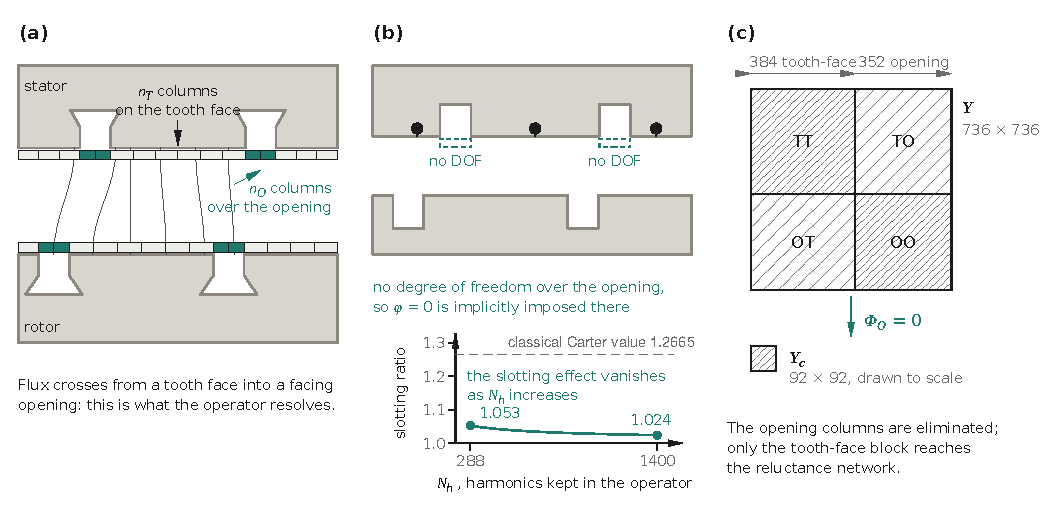
\includegraphics[width=\textwidth]{fig_gapop.pdf}
\caption{Reconstruction of the air gap for a doubly slotted annulus.
\textbf{(a)} The annulus with the tiling laid on both bores, $n_T$
columns on each tooth face and $n_O$ over each opening, and the flux
crossing from a tooth face into a facing opening. \textbf{(b)} What a
treatment without opening degrees of freedom does instead: a null
potential is imposed over the opening implicitly, and the slotting ratio
it returns collapses towards unity as the harmonic count rises, from
\num{1.053} to \num{1.024}. \textbf{(c)} The assembled operator as a
block matrix in the tooth and opening unknowns, and the Schur complement
that eliminates the opening block, drawn to scale.
Both bores are tiled by columns spanning the tooth faces and the slot
openings, so that the surface is paved exactly; the operator
\eqref{eq:Y_two} is assembled on this fine grid, where the Laplace
solution of the annulus is exact. The opening columns carry no flux into
iron, and eliminating them by the Schur complement \eqref{eq:schur_gap}
condenses the operator onto the tooth nodes of the performance network.
No fringing coefficient enters: the redistribution beneath the opening
is solved.}
\label{fig:gapop}
\end{figure*}

\begin{enumerate}[label=(\roman*),leftmargin=*]
\item the face columns of one tooth are equipotential, the tooth tip
being iron at the potential of its node, so
$\bm{U}_T=\bm{P}\,\bm{U}_{\mathrm{tooth}}$ with $\bm{P}$ a $0/1$
prolongation;
\item the opening columns deliver no flux into iron, being air, so the
flux reaching them redistributes within the annulus:
$\bm{\Phi}_O=\bm{0}$.
\end{enumerate}

Partitioning $\bm{Y}=[\bm{Y}_{TT}\;\bm{Y}_{TO};\,\bm{Y}_{OT}\;
\bm{Y}_{OO}]$ and eliminating the opening degrees of freedom gives the
Schur complement
\begin{equation}
\bm{Y}_{\mathrm{c}}=\bm{P}^{\!\top}\bigl(\bm{Y}_{TT}
-\bm{Y}_{TO}\bm{Y}_{OO}^{-1}\bm{Y}_{OT}\bigr)\bm{P},
\label{eq:schur_gap}
\end{equation}
symmetric by construction and free of any fringing parameter: the
redistribution beneath the opening is \emph{solved}, not modelled. On
the machine of Section~\ref{sec:im} the tiling $n_T=17$, $n_O=4$ reduces
a grid of $384+352$ bore columns to a dense $92\times92$ block, which is
the element the performance network sees.

Two properties of \eqref{eq:schur_gap} are worth stating because they
are what make the condensation usable. It preserves symmetry and
semi-definiteness, so the coupled nodal system remains well posed once
the iron network fixes the gauge. And it is exact on the
finite-dimensional problem: no approximation is introduced between the
fine grid and the tooth nodes. Whatever error the condensed element
carries is inherited entirely from the fine grid itself, from the
truncation of the harmonic sum and from the basis $\chi_k$ used to
represent the potential across a column. That is why the next section is
about the basis and not about the condensation.

\subsection{Reference-Free Verification of the Assembled Operator}
\label{sub:invariants}

Every comparison reported in Section~\ref{sec:im} is against a
finite-element analysis (FEA) field solution, and four constants of the performance
model are identified against that same solution
(Section~\ref{sub:identified}). A check built on such a comparison cannot
separate a correct model from an incorrect one whose error the
identification has absorbed. The case that makes this concrete rather
than rhetorical arose in the present code base, on a different machine: a
magnet-loss routine carrying a sign error in its transformation to the
rotor frame agreed with its finite-element reference to
\SI{2.4}{\percent}, while the corrected routine deviates by
\SI{-36.4}{\percent}. \emph{Agreement with
the reference was the symptom of the defect, not the test that would have
found it.}

An invariant is a check of a different kind. It is a statement the
operator must satisfy whatever the geometry, the excitation and the
discretisation, so it is verified without the reference, without
$k_{\mathrm{C}}$ and without any identified constant. Eight are available
on \eqref{eq:Y_two} and none is a convergence test: each holds at any
resolution, which is why the whole suite runs on a coarse tiling in three
seconds. Table~\ref{tab:invariants} reports it at $n_T=6$, $n_O=2$,
$N_h=\num{2048}$ in the hat basis, on the machine of
Section~\ref{sec:im}.

\begin{table*}[!t]
\centering
\begin{threeparttable}
\footnotesize
\begin{tabular}{llr@{\quad}l}
\toprule
& invariant & residual & \\
\midrule
I-1 & $\bm{Y}\,[\bm{1};\bm{1}]=\bm{0}$, no flux from a
      uniform potential & \num{9.94e-2} & fails\tnote{a}\\
I-2 & $\bm{Y}=\bm{Y}^{\!\top}$, reciprocity & \num{2.26e-16} & holds\\
I-3 & semi-definiteness, no eigenvalue of the wrong sign
                                            & \num{0} & holds\\
I-4 & homopolar permeance equal to \eqref{eq:Lam0}
                                            & \num{3.03e-3} & fails\tnote{a}\\
I-5 & torque invariant under rigid rotation & \num{1.83e-14} & holds\\
I-6 & torque zero in an aligned field       & \num{6.75e-14} & holds\\
I-7 & Maxwell stress against the energy derivative
                                            & \num{1.22e-14} & holds\\
I-8 & torque independent of the integration radius
                                            & \num{3.12e-14} & holds\\
\bottomrule
\end{tabular}
\begin{tablenotes}[flushleft]\footnotesize
\item[a] The two failures are one defect seen from two sides and are
treated in Section~\ref{sub:hatdefect}.
\item Residuals are relative. I-1 is normalised by $\max_{ij}|Y_{ij}|$
and I-4 by the analytic permeance \eqref{eq:Lam0}; I-5, I-7 and I-8 by
the torque of the test configuration, \SI{9.251049e-5}{\newton\metre},
and I-6 by the torque of the same configuration in quadrature,
\SI{7.329072e-4}{\newton\metre}.
\end{tablenotes}
\end{threeparttable}
\caption{Invariants of the assembled operator. None of the eight uses the
finite-element reference, $k_{\mathrm{C}}$, or any constant identified in
Section~\ref{sub:identified}; none is a convergence test, so each holds
at any resolution.}
\label{tab:invariants}
\end{table*}

Six hold at the level of the arithmetic, and among them I-7 deserves its
own sentence. The torque is formed twice by routes that share nothing
beyond the operator itself, once as the Maxwell stress integrated on a
circle in the gap, once as the analytic derivative of the annulus energy
\eqref{eq:W_two} with respect to rotor position, and the two agree to
\num{1.22e-14}. A finite-difference derivative does not reach that level
here and the reason is structural rather than numerical: the operator
carries content up to order $N_h$, whose angular scale $2\pi/N_h$ is of
the order of the differencing step, so the difference quotient is never
in its asymptotic regime. Writing the derivative analytically is what
makes the two routes comparable at all, and it is the form reported.

The remaining two do not hold. They are not two faults but one, seen
from two sides: both ask whether the surface basis represents the
constant function exactly, and Section~\ref{sub:hatdefect} isolates the
answer by crossing the basis against the grid.

None of this construction is specific to the doubly slotted annulus. Any
surface-to-surface map admits the same four classes of check, a null
mode, a symmetry, a conservation, and a second route to the same
output, at a cost of seconds. Where the reference is itself an object
against which constants have been fitted, they are the checks that remain
informative when comparison no longer is.

\subsection{Definition of the Slotting Ratio and of Its Comparator}
\label{sub:kcdef}

Every slotting ratio quoted in this paper is the functional
\begin{equation}
k_{\mathrm{C}}\;\equiv\;
\frac{X_{m0}^{\text{smooth}}}{X_{m0}^{\text{slotted}}},
\label{eq:kcdef}
\end{equation}
the ratio of \emph{unsaturated} magnetising reactances of two solutions
that differ in one respect only. The comparator must be stated because
it decides the number.

\emph{The smooth geometry.} Both bores are replaced by smooth cylinders
at the radii they already have---$R_s=\SI{81.8888}{\milli\metre}$ and
$R_r=\SI{81.6458}{\milli\metre}$, so the mechanical gap is unchanged at
$g=\SI{0.2430}{\milli\metre}$. The tiling, the winding, the excitation
and the harmonic truncation are those of the slotted solve. Nothing else
is altered: the iron cross-section is not preserved, the openings are
not closed at the tooth-face radius, and neither surface is smoothed
alone. Table~\ref{tab:tiling} records the control this affords, the
smooth-bore reactance is \SI{81.2698}{\ohm} at every one of the nine
tilings, invariant to \SI{0.00}{\percent}, because a bore without
openings has nothing for the tiling to resolve.

\emph{What \eqref{eq:kcdef} is, and is not.} Carter's factor is defined
as an effective-gap ratio $g_{\text{eff}}/g$: the gap of a smooth
machine having the same fundamental air-gap permeance. Equation
\eqref{eq:kcdef} is a reactance ratio at fixed winding and fixed
excitation. The two coincide when $X_{m0}$ is proportional to the
air-gap permeance, which requires the comparison to be unsaturated and
linear, it is both, $X_{m0}$ being used throughout, the winding
distribution to be identical between the two solves, which the
construction above guarantees; \emph{and the iron reluctance to be
negligible beside the air-gap reluctance in both solves}. Under those
three conditions \eqref{eq:kcdef} and Carter's ratio measure the same
thing, and outside them they do not.

\emph{The third condition is not met on this machine, and the amount by
which it is not met is measured.} Both unsaturated solves are taken on
the real $B(H)$ curve at a common low excitation, so the permeability is
finite and \emph{identical} on the two sides, between
$\mu_{\mathrm{r}}=\num{1507}$ at \SI{0.2}{\tesla} and
$\num{3808}$ at \SI{1.0}{\tesla}. Repeating both solves at
$\mu_{\mathrm{r}}=\num{1e5}$, with the operator, the tiling
$n_T=17$, $n_O=4$, the truncation $N_h=\num{8192}$ and the excitation
all unchanged, gives
\begin{equation}
\begin{aligned}
X_{m0}^{\text{smooth}} &: \;\SI{81.2698}{\ohm}\rightarrow\SI{181.8592}{\ohm},\\
X_{m0}^{\text{slotted}} &: \;\SI{61.0147}{\ohm}\rightarrow\SI{113.4772}{\ohm},\\
k_{\mathrm{C}} &: \;\num{1.3320}\rightarrow\num{1.6026},
\end{aligned}
\label{eq:muinf}
\end{equation}
a displacement of \SI{+20.3}{\percent}, three times the tiling
dispersion of \SI{6.82}{\percent} that Section~\ref{sub:tilesens}
reports. That the smooth-bore reactance itself more than doubles is the
direct evidence: if the iron carried a negligible reluctance it would
not move at all.

\emph{What this does and does not change.} It does not touch the
direction of the result. A series iron reluctance $\rho$ common to both
solves returns $(k_{\mathrm{C}}+\rho)/(1+\rho)$, which is compressed
\emph{towards unity}: every ratio this paper reports is therefore a
\emph{lower} bound on the air-gap ratio, and the one-sided claim that
the classical value is low in this regime is strengthened rather than
weakened, the excess over \num{1.2665} would be \SI{26.6}{\percent}
at infinite iron against \SI{5.2}{\percent} at the production tiling.
What it does change is the reading of the interval: \emph{the values
reported here are ratios of a network in which the iron participates,
not of the annulus alone}, and the quantity Carter's factor is defined
to be is the infinite-iron one. Which of the two a corrected coefficient
should carry is left open, because settling it displaces every value
in Sections~\ref{sec:p1} to~\ref{sec:carter} and is a question about
what the coefficient is for, not about what the operator returns.

\emph{One further asymmetry must be declared.} Carter's value for a
doubly slotted machine is the \emph{product} of two per-surface factors,
each derived for one slotted surface facing a smooth one. The operator
returns a \emph{joint} quantity, obtained with both surfaces slotted at
once. The comparison of Section~\ref{sec:carter} is therefore between
two different constructions of the same design coefficient, not between
two evaluations of one construction. That is the point of the exercise,
and it is also its principal caveat.

\subsection{Carter's Value for This Machine}
\label{sub:carterval}

The classical value this paper compares against is reproduced here in
full, so that a reader can check it. With
\begin{equation}
\gamma=\frac{(b_0/g)^2}{5+b_0/g},
\qquad
k_{\mathrm{C}}^{\text{surf}}=\frac{\tau}{\tau-\gamma g},
\label{eq:carterform}
\end{equation}
the approximate form given by~\cite{carter,pyrhonen}, and the dimensions
read from the finite-element project:

\begin{center}\footnotesize
\begin{tabular}{lrr}
\toprule
 & stator & rotor \\
\midrule
slot opening $b_0$ (\si{\milli\metre}) & 2.0000 & 2.0000 \\
gap $g$ (\si{\milli\metre})            & 0.2430 & 0.2430 \\
slot pitch $\tau$ (\si{\milli\metre})  & 10.7192 & 11.6590 \\
$b_0/g$                                & 8.2305 & 8.2305 \\
$\gamma$                               & 5.120033 & 5.120033 \\
$k_{\mathrm{C}}^{\text{surf}}$           & 1.131310 & 1.119461 \\
\midrule
\multicolumn{3}{l}{product $k_{\mathrm{C}}^{\text{Carter}}
 = \num{1.266458}$}\\
\bottomrule
\end{tabular}
\end{center}

\vspace{2mm}

The exact conformal-mapping form,
$\gamma=(4/\pi)\left[x\arctan x-\ln\sqrt{1+x^2}\right]$ with
$x=b_0/2g$, gives \num{1.267924} instead, a difference of
\SI{0.12}{\percent}. \emph{The approximate form is the one used
throughout this paper}, because it is the one the comparison model
implements; the exact form is quoted so that the choice is visible and
so that a reader reproducing \num{1.2665} by the other route knows why
the last digit differs.


%=======================================================================
\section{Convergence in the Hat Basis}
\label{sec:p1}

The condensation of Section~\ref{sec:twosurface} is exact on the
continuous problem; what is condensed in practice is its restriction to
a finite-dimensional space of surface potentials, and that restriction
is not innocent. Appendix~\ref{app:trace} establishes the point in
closed form: the self-energy of a piecewise-constant surface column grows as
$\ln N$ without bound, because a function with jumps does not belong to
$H^{1/2}(\Gamma)$, the trace space on which the operator is bounded;
the continuous piecewise-linear (hat) basis does belong to it and
restores an absolutely convergent series, with a residual tail in
$1/N^{2}$. This section carries that result over to the doubly slotted
annulus and measures its consequence.

Table~\ref{tab:kc} sweeps the truncation at fixed tiling, $n_T=17$
columns per tooth face, $n_O=4$ per slot opening, the operator condensed
onto 92 tooth nodes, in both bases, and reports the magnetising
reactance of the same annulus with and without slotting.

Three readings, in increasing order of consequence. First, the
smooth-bore column is rigorously constant in the hat basis,
\SI{81.270}{\ohm} at every truncation, against a \SI{0.15}{\percent}
drift in the piecewise-constant basis, the hat basis represents a
jump-free potential exactly, so a smooth bore has nothing left for the
truncation to resolve. Second, on the slotted geometry the drift is
\SI{5.99}{\percent} in the piecewise-constant basis against
\SI{0.62}{\percent} in the hat basis, forty times the drift of the
smooth bore, on the same sweep and the same tiling. Third, and this is
the number that carries Section~\ref{sec:carter}: that ratio of
\num{40} between numerator and denominator is what makes the slotting
ratio inherit the drift of its denominator essentially in full.

The converged value is
\begin{equation}
X_{m0}=\SI{61.015}{\ohm}\quad\text{at }N_h=\num{8192},
\label{eq:xm0}
\end{equation}
and the \emph{dispersion} of the derived slotting ratio, its range
divided by its mean over the sweep, falls from \SI{5.68}{\percent} to
\SI{0.62}{\percent} between the two bases. Truncation has become a
choice of precision.

Two statistics are used in this paper and they are not the same number.
The \emph{drift} is the end-to-end relative change across a sweep, and
it is what the last row of Table~\ref{tab:kc} reports; the
\emph{dispersion} is the range divided by the mean, and it is what the
text quotes when a sweep is not monotone. On the piecewise-constant
slotting ratio they differ---\SI{-5.51}{\percent} against
\SI{5.68}{\percent}, because the drift is normalised by the first
value and the dispersion by the mean; on a monotone sequence the first
value is an extremum, so the dispersion is the larger of the two. Each
is named explicitly wherever it appears.

\begin{table*}[!t]
\centering
\begin{threeparttable}
\footnotesize
\begin{tabular}{rrrrrrr}
\toprule
& \multicolumn{3}{c}{piecewise constant} & \multicolumn{3}{c}{hat}\\
\cmidrule(lr){2-4}\cmidrule(lr){5-7}
$N_h$ & $X_m$ smooth & $X_m$ slotted & $k_{\mathrm{C}}$
      & $X_m$ smooth & $X_m$ slotted & $k_{\mathrm{C}}$\\
      & (\si{\ohm}) & (\si{\ohm}) & & (\si{\ohm}) & (\si{\ohm}) & \\
\midrule
\num{512}  & \num{81.912} & \num{61.900} & \num{1.3233} & \num{81.270} & \num{60.639} & \num{1.3402}\\
\num{1024} & \num{81.944} & \num{63.094} & \num{1.2988} & \num{81.270} & \num{60.954} & \num{1.3333}\\
\num{2048} & \num{81.973} & \num{64.038} & \num{1.2801} & \num{81.270} & \num{60.998} & \num{1.3323}\\
\num{4096} & \num{82.003} & \num{64.863} & \num{1.2642} & \num{81.270} & \num{61.011} & \num{1.3321}\\
\num{8192} & \num{82.032} & \num{65.607} & \num{1.2503} & \num{81.270} & \num{61.015} & \num{1.3320}\\
\midrule
drift & $+0.15\%$ & $+5.99\%$ & $-5.51\%$ & $+0.00\%$ & $+0.62\%$ & $-0.62\%$\\
\bottomrule
\end{tabular}
\begin{tablenotes}[flushleft]\footnotesize
\item Tiling $n_T=17$,
$n_O=4$; operator condensed to $92\times92$; classical Carter value for
this geometry \num{1.2665}.
\end{tablenotes}
\end{threeparttable}
\caption{Truncation sweep of the doubly slotted operator in both surface
bases, at fixed tiling. The smooth-bore column is rigorously constant in
the hat basis; the ratio of the two piecewise-constant drifts is
\num{40}.}
\label{tab:kc}
\end{table*}

\subsection{A Measured Defect of the Hat Basis on the Tiled Grid}
\label{sub:hatdefect}

The two invariants that fail in Table~\ref{tab:invariants} fail on the
configuration this paper retains, and they fail together. I-1 asks
whether a uniform potential drives any flux and I-4 whether the operator
returns the analytic homopolar permeance \eqref{eq:Lam0}; both are
consequences of one property, \emph{that the surface basis represent the
constant function exactly}, and crossing the basis against the grid
isolates it without ambiguity. Table~\ref{tab:hatdefect} does that.

\begin{table}[!ht]
\centering
\begin{threeparttable}
\footnotesize
\setlength{\tabcolsep}{4pt}
\begin{tabular}{llrr}
\toprule
\multicolumn{4}{l}{(a) basis against grid, at $N_h=\num{2048}$}\\
\midrule
basis & grid & I-1 & I-4\\
\midrule
piecewise constant & tiled   & \num{1.57e-12} & \num{1.24e-16}\\
hat                & tiled   & \num{9.94e-2}  & \num{3.03e-3}\\
piecewise constant & uniform & \num{2.69e-14} & \num{2.48e-16}\\
hat                & uniform & \num{6.23e-15} & \num{1.24e-16}\\
\midrule
\multicolumn{4}{l}{(b) I-4 against the truncation, on the tiled grid}\\
\midrule
\multicolumn{2}{l}{$N_h$} & hat & piecewise constant\\
\midrule
\multicolumn{2}{l}{\num{256}}  & \num{8.78e-4} & \num{2.48e-16}\\
\multicolumn{2}{l}{\num{1024}} & \num{2.88e-3} & \num{1.24e-16}\\
\multicolumn{2}{l}{\num{4096}} & \num{3.04e-3} & \num{2.48e-16}\\
\bottomrule
\end{tabular}
\begin{tablenotes}[flushleft]\footnotesize
\item Residuals as in Table~\ref{tab:invariants}. \emph{Tiled} is the
grid of Section~\ref{sub:tiling}, in which tooth-face and opening columns
have different widths; \emph{uniform} is the same number of columns at
equal width.
\end{tablenotes}
\end{threeparttable}
\caption{The defect crossed against its two factors. The
piecewise-constant basis holds the property on both grids; the hat basis
holds it on the uniform grid and loses it on the tiled one, which is the
grid of production. Panel (b) shows that refinement does not remove it.}
\label{tab:hatdefect}
\end{table}

Four statements follow, and the order matters because the third is the
one most easily over-read.

\emph{What is established.} On the homopolar mode the annulus permeance
the operator returns, \SI{4.391224e-4}{\henry}, stands
\SI{+0.303}{\percent} from its analytic value
$\mu_0\,2\pi L/\Xg=\SI{4.377977e-4}{\henry}$, and a potential raised
uniformly on both surfaces drives a flux that should be rigorously zero.
Neither is a matter of precision: panel (b) shows the discrepancy
\emph{growing} with the truncation and then saturating, where truncation
error would fall. Refining $N_h$ does not remove it, and no choice of
$N_h$ would have exposed it either, which is why an invariant was needed
to find it at all.

\emph{The cause.} A hat of half-width $h$ tiles the circle only if the
half-widths agree from one column to the next. The tiling of
Section~\ref{sub:tiling} uses \emph{deliberately} different widths for
the columns spanning a tooth face and those spanning a slot opening: that difference is the reason the tiling exists. At each face-to-opening
junction the neighbouring hats therefore leave a gap or an overlap, the
basis sums to something other than one there, and the constant function
is no longer in its span. The piecewise-constant basis paves the circle
by construction whatever the widths, and keeps the property: \emph{this
is the one measured quantity on which it is superior to the hat basis},
and it is stated here as neither more nor less than that.

\emph{What is not established.} Whether this bias propagates to
$k_{\mathrm{C}}$ or to $X_m$, and by how much. I-1 and I-4 are posed on
the homopolar mode and measure the homopolar mode; the slotting ratio is
formed from the orders $n\ge1$, on which neither test says anything. \emph{No propagation is inferred here}, in either direction: the
question requires its own measurement, and the only clean way to obtain
it is to correct the basis and recompute, which displaces every published
value of this paper and is therefore reported rather than performed.

\emph{The remedy, which is analytic.} An \emph{asymmetric} hat, whose
left and right half-widths are the local half-steps of the grid rather
than a common $h$, restores the partition of unity on an arbitrary grid.
Its Fourier projection stays in closed form: an asymmetric hat is the
convolution of two rectangles of unequal width, so its transform is the
product of their transforms with a phase term, and \eqref{eq:app_p1}
generalises without leaving the closed-form setting that makes the
assembly cheap. The change is confined to the projection $W_n$; the
condensation \eqref{eq:schur_gap} and everything downstream of it are
untouched.

One qualification belongs with all four. The argument this paper makes
for the hat basis is its membership of $H^{1/2}(\Gamma)$ and the
$1/n^{2}$ decay of its projection, the reason the energy series
converges at all, set out in Appendix~\ref{app:trace}, and that argument
is untouched by the defect above, which concerns the representation of
one mode and not the summability of the series. \emph{The hat basis
remains the retained basis, and the reason it is retained is unchanged.}

%=======================================================================
\section{A Quantified Correction to Carter's Factor}
\label{sec:carter}

At the production tiling $n_T=\num{17}$, $n_O=\num{4}$, the
converged-basis slotting ratio of Table~\ref{tab:kc} is
\begin{equation}
k_{\mathrm{C}}=\num{1.3320}
\qquad\text{against}\qquad
k_{\mathrm{C}}^{\text{Carter}}=\num{1.2665},
\label{eq:kc}
\end{equation}
that is \SI{+5.2}{\percent}. \emph{This is the value at one
discretisation and not a property of the geometry}: Table~\ref{tab:tiling}
shows the ratio still moving with the tiling, and the result this paper
claims is the interval of Section~\ref{sub:tilesens}, not \eqref{eq:kc}.
An earlier version of this work reported
that the operator reproduced Carter's ratio to three decimals, and
presented that agreement as a validation. It was not one, and the
present section explains why the correction is the more interesting
result.

\subsection{The Three-Decimal Agreement as a Truncation Coincidence}
\label{sub:kccoincidence}

An earlier version of this work reported that the operator reproduced
Carter's ratio to three decimals, and offered that agreement as a
validation. It was not one, and the reason is visible only once the
truncation is swept: the curve crosses the classical value on its way
past it. Withdrawing that claim is what makes the correction below
reportable.

Read the piecewise-constant column of Table~\ref{tab:kc} downwards:
\num{1.3233}, \num{1.2988}, \num{1.2801}, \num{1.2642}, \num{1.2503}.
The curve crosses Carter's \num{1.2665} between $N_h=\num{2048}$ and
$N_h=\num{4096}$ and keeps falling; at $N_h=\num{8192}$ it stands at
\num{1.2503} and shows no sign of settling. The successive increments of
that column, formed from the four decimals printed in
Table~\ref{tab:kc}, are \num{-0.0245}, \num{-0.0187}, \num{-0.0159} and
\num{-0.0139}, in ratios \num{0.76}, \num{0.85} and \num{0.87}:
\emph{ratios climbing towards unity are the signature of a logarithmic
tail}, whereas a convergent sequence settles at a ratio below one
(Appendix~\ref{app:trace}). \emph{The agreement was obtained by stopping the
sweep where the curve happened to cross.} Any other truncation would
have given another number, and the sweep itself shows that there is no
limit to converge to.

\subsection{Physical Basis for Exceeding the Classical Value}
\label{sub:priorwork}

Carter's construction~\cite{carter} maps a \emph{single, isolated} slot
in an infinite half-plane by conformal transformation. Its accuracy has
been examined before, and the existing assessments frame what is claimed
here. Viorel \emph{et al.}~\cite{viorel2007} compare the closed-form
expressions in circulation against finite-element computation and report
that they do not agree with one another, the spread widening as the
opening grows; the same authors later confirm the trend on a wider set
of geometries~\cite{viorel2014}. Working from the field rather than from
the factor, Bannae Sharifian \emph{et al.}~\cite{sharifian2003} extract
the fringing coefficient by finite elements and propose a modified
coefficient because the classical curve departs from the computed field
at large openings. Two features are common to these studies and to every
other assessment we are aware of: the reference is a finite-element
\emph{field}, from which a factor is inferred by a chosen definition,
and the geometry corrected is a \emph{single} slotted surface. Neither
returns the ratio directly, and neither addresses the doubly slotted
case. Two of Carter's hypotheses fail on this machine. The slot opening is not small compared
with the gap, here
\begin{equation}
\frac{b_0}{g}=\frac{\SI{2.000}{\milli\metre}}{\SI{0.243}{\milli\metre}}
=\num{8.23},
\label{eq:b0g}
\end{equation}
so neighbouring slots interact through the gap instead of each
perturbing an otherwise uniform field. And \emph{both} surfaces are
slotted, whereas the classical treatment corrects one surface at a time
and multiplies the two factors, an approximation that has no
justification when the two slot pitches are comparable and the gap is
thin. That the two slottings interact instead of superpose is not in
doubt, dynamic models that carry both slot sets explicitly reproduce
air-gap harmonics that neither surface produces alone~\cite{nandi2003}, but
those models return a field, and the product $k_{Cs}k_{Cr}$ has
continued to be used for the permeance because no alternative closed
quantity was available. The doubly slotted operator resolves both effects by construction,
because it solves the annulus instead of correcting it.

That an exact solution of the annulus should return more than Carter in
this regime is therefore expected. What is new is the \emph{amount}: a
quantified correction to a century-old result, obtained with no fitted
coefficient anywhere in the chain. That is a contribution;
``we recover Carter'' was not one, since it taught nothing that Carter
did not already say.

\subsection{Sensitivity to the Tiling, and What It Leaves Established}
\label{sub:tilesens}

The truncation is not the only discretisation the ratio depends on. The
two bores are tiled, and Section~\ref{sub:tiling} states that without a
tiling the ratio tends to unity: the tiling is not an implementation
detail but what makes the effect exist. It must therefore carry its own
sensitivity study, and it does not survive it as the truncation does.

Table~\ref{tab:tiling} sweeps the tooth-face and opening subdivisions
over a factor of four each, at fixed $N_h=\num{8192}$ in the hat basis.
The smooth-bore reactance is invariant, \SI{81.2698}{\ohm} at every
point. The slotted reactance is not: it rises monotonically in
\emph{both} refinement directions, from \SI{58.51}{\ohm} to
\SI{62.62}{\ohm}, and does not settle. The ratio inherits that drift
essentially in full---dispersion \SI{6.82}{\percent} on $k_{\mathrm{C}}$
against \SI{6.75}{\percent} on its denominator, so the guard that would
have rescued the result, the ratio being better conditioned than its
parts, fails.

Three consequences must be stated rather than absorbed.

\emph{First, the dispersion is of the same order as the correction.} The
excess over Carter's value ranges from \SI{+9.67}{\percent} at the
coarsest tiling to \SI{+2.48}{\percent} at the finest, against
\SI{+5.2}{\percent} at the production tiling. A reader is entitled to
observe that the correction and its discretisation uncertainty are not
separated.

\emph{Second, the finest point is not a converged value but a lower
bound.} The slotted reactance is still rising and $k_{\mathrm{C}}$ still
falling at the finest tiling computed. Nothing in these data excludes
that further refinement brings $k_{\mathrm{C}}$ back to, or below,
Carter's value.

\emph{Third, this is the defect of Section~\ref{sec:p1} transposed to a
second axis.} There, a quantity was shown to have no limit under
truncation refinement because the trial space was non-conformal, and the
remedy was a conforming basis. Here the same symptom appears along the
tiling axis, and the present paper does not establish that a limit
exists. The two axes are not equivalent, the truncation defect was
proved in closed form, whereas this one is observed, but the reader
should not be asked to accept the second on the strength of the first.

What survives is therefore narrower than a corrected value of Carter's
factor, and it should be read as such. Over a factor of four in each
tiling direction, in a regime where Carter's hypotheses are violated by
construction, the converged-basis ratio exceeds the classical value at
\emph{every one of the nine points computed}, by between
\SI{2.5}{\percent} and \SI{9.7}{\percent}. That the classical value is
low here is established. \emph{By how much is not}, and the figure
\SI{+5.2}{\percent} should be read as the value at one declared tiling
rather than as a property of the geometry. Establishing the latter
requires the tiling axis to be closed as the truncation axis was, and
that is left to further work.

\emph{One further bound belongs on the engineering claim.} The ratio
defined by \eqref{eq:kcdef} is an \emph{unsaturated} slotting ratio: it
is formed on $X_{m0}$, by construction and correctly, since Carter's
factor is itself a linear-permeance quantity. The design use of that
factor is however to set the operating flux level and hence tooth
saturation. Section~\ref{sub:im_tests} shows that the two cannot be
reconciled by a single scaling, raising the unsaturated reactance
enough to correct the no-load current would also raise the saturated
value, which is already \SI{10.6}{\percent} \emph{below} the reference
and would then overshoot it. \emph{The corrected ratio therefore cannot
be substituted into a classical saturated design chain by rescaling
$X_m$}, and at least one further mechanism is present. This bounds what
the result licenses without weakening the physics behind it.

\begin{table*}[!tb]
\centering
\begin{threeparttable}
\footnotesize
\begin{tabular}{rrrrrr}
\toprule
$n_T$ & $n_O$ & columns & $X_m$ slotted (\si{\ohm})
      & $k_{\mathrm{C}}$ & dev.\ from production \\
\midrule
\num{9}  & \num{2} & \num{1012} & \num{58.5130} & \num{1.3889} & $+4.28\%$\\
\num{9}  & \num{4} & \num{1196} & \num{59.8667} & \num{1.3575} & $+1.92\%$\\
\num{9}  & \num{8} & \num{1564} & \num{60.8360} & \num{1.3359} & $+0.29\%$\\
\num{17} & \num{2} & \num{1748} & \num{59.7955} & \num{1.3591} & $+2.04\%$\\
\textbf{\num{17}} & \textbf{\num{4}} & \textbf{\num{1932}}
     & \textbf{\num{61.0147}} & \textbf{\num{1.3320}} & \textbf{---}\\
\num{17} & \num{8} & \num{2300} & \num{61.9376} & \num{1.3121} & $-1.49\%$\\
\num{33} & \num{2} & \num{3220} & \num{60.9017} & \num{1.3344} & $+0.19\%$\\
\num{33} & \num{4} & \num{3404} & \num{61.9532} & \num{1.3118} & $-1.51\%$\\
\num{33} & \num{8} & \num{3772} & \num{62.6202} & \num{1.2978} & $-2.56\%$\\
\bottomrule
\end{tabular}
\begin{tablenotes}[flushleft]\footnotesize
\item Hat basis, $N_h=\num{8192}$ at every point. The smooth-bore
reactance is \SI{81.2698}{\ohm} throughout, invariant by construction.
Dispersion: \SI{0.00}{\percent} on the numerator, \SI{6.75}{\percent} on
the denominator, \SI{6.82}{\percent} on the ratio. Carter's value for
this geometry is \num{1.2665}; every row exceeds it.
\end{tablenotes}
\end{threeparttable}
\caption{Sensitivity of the slotting ratio to the surface tiling. The
ratio is not better conditioned than its denominator, and neither has
converged over the range computed.}
\label{tab:tiling}
\end{table*}

\subsection{Invalidity of the Compensation Argument}

An earlier version defended the classical value by arguing that the
truncation bound affects numerator and denominator alike and therefore
largely cancels in the ratio. Table~\ref{tab:kc} refutes this by direct
reading, in two columns. Over the same sweep, in the piecewise-constant
basis, the numerator, the smooth-bore reactance, drifts by
\SI{0.15}{\percent} while the denominator, the slotted
reactance, drifts by \SI{5.99}{\percent}. The ratio of the two drifts
is \num{40}. \emph{The ratio inherits the drift of its denominator
essentially in full}, and no cancellation takes place. The hat basis
removes the drift from both: \SI{0.00}{\percent} and
\SI{0.62}{\percent}.

The mechanism is the one Section~\ref{sec:p1} names. The smooth bore
carries no potential jump, so the piecewise-constant basis represents it
almost exactly and its residual drift measures only projection error.
The slotted bore carries a jump at every slot opening, that is what a
slot opening \emph{is}, seen from the surface potential, so the
piecewise-constant basis is non-conformal precisely where the physics
lives.

%=======================================================================
\section{Validation: 18.5\,kW Cage Induction Machine}
\label{sec:im}

\subsection{Protocol, Information Sources and Data Extraction}
\label{sub:im_protocol}

The comparison follows a protocol fixed before the runs, and what
follows is specific to this machine. No registration
is claimed, for want of a registry that would accept a study of this
kind; the instrument used in its place is a dated manifest kept with the
code, which names for every published quantity the chain producing it,
the transcript it is read from and the configuration that defines it. The repository
holds \num{37} executable run scripts for this machine, of which
\num{16} write such a transcript, so the manifest is what makes a
published cell traceable at all: nothing in the file system itself
distinguishes a chain that fed a table from one that did not. No value is transcribed by hand, every deviation
is formed on full-precision values and rounded once at display, a table
is filled from a transcript and never from another table, and where a
transcript holds several solved blocks it is the last \emph{complete}
one, checked for internal consistency, not merely last, that is
authoritative.

What must be declared for this machine is wider than the geometry,
because the numerical state is part of the specimen: the tiling of the
two bores, the harmonic truncation, the surface basis and the state of
the skew reduction all change the answer, and each table below names
them. The comparator is a named finite-element study rather than the
project, since this project returns the same physical quantity by two
routes of unequal resolution; Section~\ref{sub:im_ec} states which route
each row uses and why a single family is used throughout.

Three exclusions apply and are recorded rather than left to be inferred.
The parametric slip sweep is not used as a reference above
$s=\num{0.90}$, where its scatter reaches \SI{16}{\percent} of the local
mean, the dedicated transient run being used instead. The standstill row
is removed from the balance of Section~\ref{sub:im_ec} and treated on
its own in Section~\ref{sub:standstill}, because at $s=1$ the harmonic
cage governs the result and the row would otherwise be read as a verdict
on the closure. And the breakdown torque is reported as a faithful
transcription of a point in the clean band, not as a verified maximum,
for the reason given with Fig.~\ref{fig:im_char}: the largest value in
the file lies inside a band whose local scatter is \SI{13}{\percent}.

That figure collects the slip-dependent behaviour, and its panels should
be identified before the argument is made from them. Panel~(a) gives the
raw torque--slip sweep of the reference, plotted point by point rather
than smoothed, with the band over which the point-to-point roughness
stays low marked on it; panel~(b) the corresponding current--slip
characteristic; panel~(c) the efficiency and the power factor, the two
quantities a designer reads first; and panel~(d) the loss breakdown
computed by the network, which attributes the efficiency of panel~(c) to
mechanisms. The argument of the preceding paragraph rests on panel~(a)
alone: it is because the raw points are shown that the scatter can be
quoted, and a smoothed curve would have concealed exactly the quantity
that disqualifies the breakdown torque as a verified maximum.

\begin{figure*}[!tb]
\centering
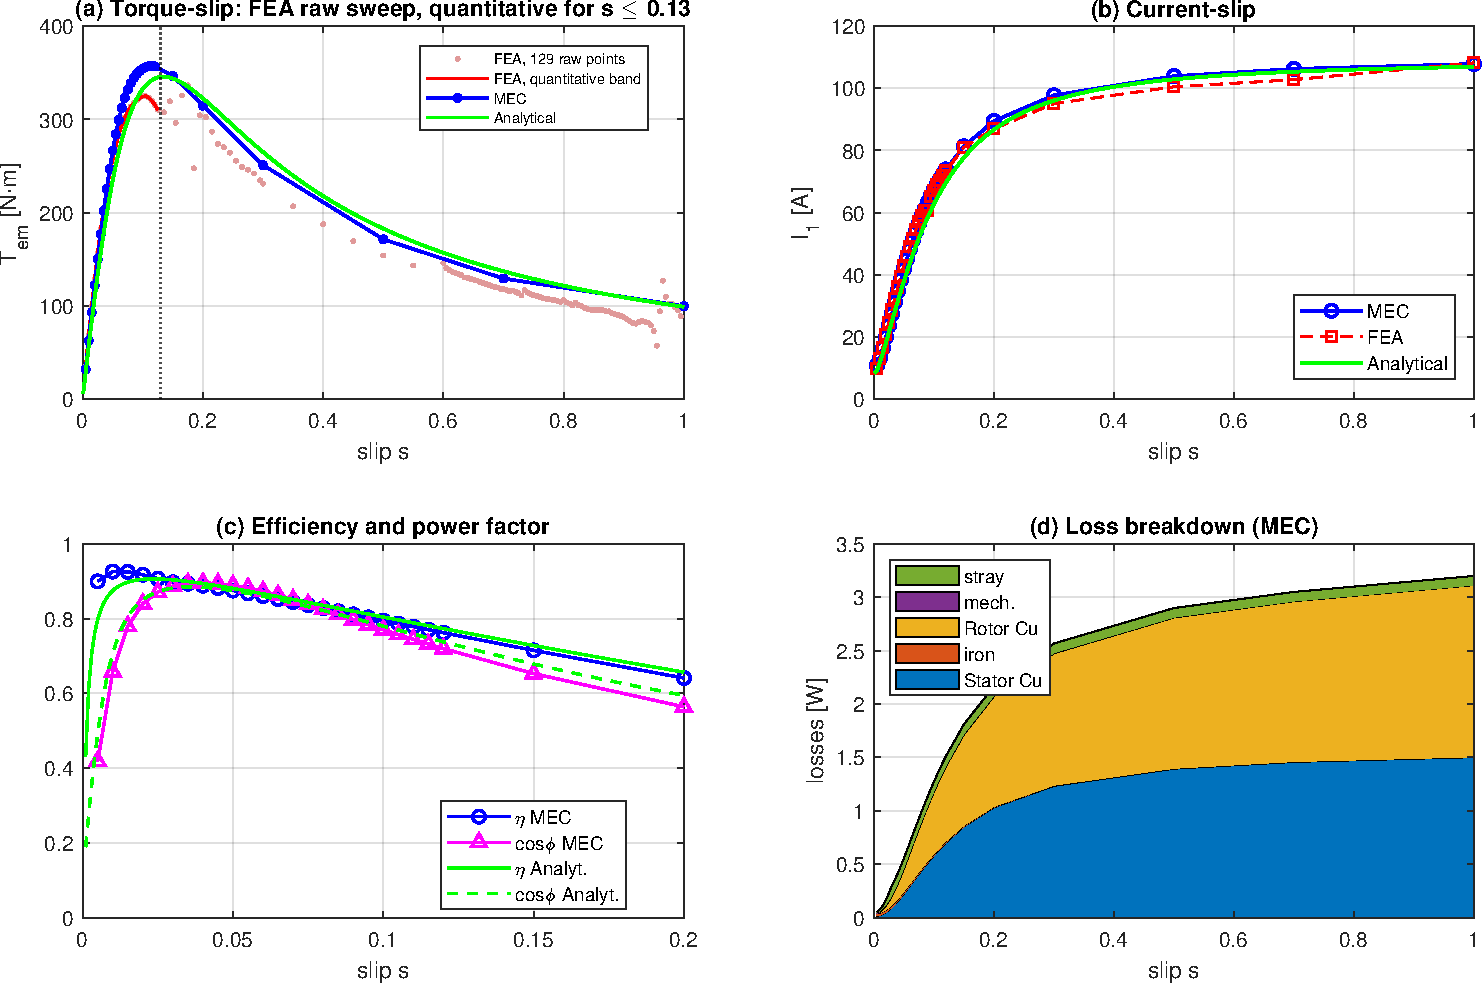
\includegraphics[width=\textwidth,height=0.44\textheight,keepaspectratio]{article_II_caracteristiques.pdf}
\caption{Slip-dependent behaviour of the \SI{18.5}{\kilo\watt} machine.
\textbf{(a)} Torque--slip sweep of the reference, plotted point by point
rather than smoothed, with the quantitative band marked.
\textbf{(b)} Current--slip characteristic. \textbf{(c)} Efficiency and
power factor. \textbf{(d)} Loss breakdown computed by the network, which
attributes the efficiency of panel~(c) to mechanisms. The
finite-element points of panel~(a) are the time-averaged torque of a parametric slip
sweep, plotted raw: the solid band $s\le\num{0.13}$ is the region whose
point-to-point roughness stays below \SI{0.7}{\percent} and which is
used quantitatively; the lighter points beyond it scatter by
\SIrange{9}{13}{\percent} and are shown so that the restriction can be
seen instead of taken on trust. The breakdown point carries a
reservation of the same kind: the value \SI{324.9}{\newton\metre} at
$s=\num{0.105}$ belongs to the clean band and is a faithful reading of
the sweep, but it is not verifiable \emph{as a maximum}, the largest
value in the file, \SI{336.6}{\newton\metre} at $s=\num{0.175}$, lies
inside a band whose local scatter is \SI{13}{\percent}. Any comparison
of the model's breakdown torque with this figure inherits that
reservation.}
\label{fig:im_char}
\end{figure*}

Two chains coexist in the results below and are not interchangeable. The
performance network condenses the annulus operator in the hat basis at
the truncation stated with each table; the local probes of the refined
mesh call a separate air-gap routine, in the piecewise-constant basis
and at a far coarser truncation. The consequence is measured rather than
assumed, and Section~\ref{sub:im_fields} reports it; the probes are
labelled accordingly wherever they appear.

\emph{Two limitations attach to the probe comparison and belong
together, since either alone understates it.} The probe chain is
\emph{unconverged}, it drifts by up to \SI{5.55}{\percent} under a
factor-of-eight truncation sweep, worst on the rotor tooth. And its
eight reference values are maxima \emph{read from field maps} rather
than exported quantities, so they are not re-derivable. The comparison
is therefore neither converged on one side nor reproducible on the
other, and any inference drawn from it, including the residual-error
lead of Section~\ref{sub:im_tests}, is a hypothesis rather than a
result. Re-running the probes in the production basis and truncation
would remove the first limitation but not the second.

Deviations are quoted as signed relative differences with respect to the
finite-element value, negative meaning that the network is below it,
except for efficiency and power factor, which are compared as
differences in points. No aggregate is formed across the quantities of a
table. They are different functionals of the same two field solutions
and are related to one another by construction, so a pooled deviation or
a dispersion statistic computed over them would impose a sampling
structure the set does not have. Where a quantity depends on a numerical
choice, the dependence is reported as such: the invariance of the
magnetising reactance to surface refinement is measured in
Section~\ref{sub:identified}, its convergence in the truncation in
Section~\ref{sec:p1}, and the cost of the skew setting in
Section~\ref{sub:standstill}.

\subsection{Machine Specification, Reference Solution and Scope}
\label{sub:im_scope}

The machine is an \SI{18.5}{\kilo\watt}, \SI{690}{\volt}, four-pole cage
induction motor with 48 stator slots and 44 rotor bars, M800-50A
laminations, a semi-closed trapezoidal stator slot and a shouldered
rotor slot. Its geometry, winding and material data are read from the
finite-element project rather than transcribed, and they are given in
full in Table~\ref{tab:machine} so that every quantity of this paper can
be recomputed from the paper alone.

\begin{table*}[!t]
\centering
\begin{threeparttable}
\footnotesize
\setlength{\tabcolsep}{3pt}
\begin{tabular}{@{}lrl@{}}
\toprule
Quantity & Value & Unit\\
\midrule
\multicolumn{3}{@{}l}{\emph{Ratings}}\\
Rated output $P_{\mathrm{n}}$              & \num{18.5} & \si{\kilo\watt}\\
Line voltage $U_{\ell\ell}$, star          & \num{690} & \si{\volt}\\
Supply frequency $f$                       & \num{50} & \si{\hertz}\\
Pole pairs $p$ / phases $m$                & \num{2} / \num{3} & ---\\
\midrule
\multicolumn{3}{@{}l}{\emph{Geometry}}\\
Active length $L$                          & \num{164.7824} & \si{\milli\metre}\\
Mechanical gap $g$                         & \num{0.243} & \si{\milli\metre}\\
Stator bore $D_{\mathrm{s}}$               & \num{163.7775} & \si{\milli\metre}\\
Stator outer diameter $D_{\mathrm{so}}$    & \num{266.5506} & \si{\milli\metre}\\
Rotor outer diameter $D_{\mathrm{r}}$      & \num{163.2915} & \si{\milli\metre}\\
Shaft diameter $D_{\mathrm{sh}}$           & \num{74.2665} & \si{\milli\metre}\\
Stacking factor $k_{\mathrm{Fe}}$          & \num{0.97} & ---\\
Stator slots / rotor bars                  & \num{48} / \num{44} & ---\\
Slot pitch $\tau_{\mathrm{s}}$ / $\tau_{\mathrm{r}}$ & \num{10.7192} / \num{11.6590} & \si{\milli\metre}\\
Stator / rotor yoke depth                  & \num{20.838} / \num{22.801} & \si{\milli\metre}\\
\midrule
\multicolumn{3}{@{}l}{\emph{Stator slot, semi-closed trapezoidal}}\\
Opening $b_{\mathrm{s}0}$                  & \num{2.000} & \si{\milli\metre}\\
Widths $b_{\mathrm{s}1}$, $b_{\mathrm{s}2}$ & \num{5.2360} / \num{8.4724} & \si{\milli\metre}\\
Heights $h_{\mathrm{s}0}$, $h_{\mathrm{s}1}$, $h_{\mathrm{s}2}$ & \num{0.50} / \num{2.50} / \num{24.7242} & \si{\milli\metre}\\
\midrule
\multicolumn{3}{@{}l}{\emph{Rotor slot, shouldered}}\\
Opening $b_{\mathrm{r}0}$                  & \num{2.000} & \si{\milli\metre}\\
Circles $b_{\mathrm{r}1}$, $b_{\mathrm{r}2}$ & \num{5.8043} / \num{2.0382} & \si{\milli\metre}\\
Isthmus height / circle spacing            & \num{1.00} / \num{16.7898} & \si{\milli\metre}\\
Bar / end-ring section                     & \num{80.70} / \num{565.12} & \si{\milli\metre\squared}\\
\midrule
\multicolumn{3}{@{}l}{\emph{Winding}}\\
Conductors per coil side $N_{\mathrm{tc}}$ & \num{18} & ---\\
Layers / parallel paths                    & \num{2} / \num{2} & ---\\
Coil pitch $y_q$ (full pitch \num{12})     & \num{10} & slots\\
Fundamental winding factor $k_{w1}$        & \num{0.9250} & ---\\
Series turns per phase $N_{\mathrm{ph}}$   & \num{144} & ---\\
\midrule
\multicolumn{3}{@{}l}{\emph{Materials}}\\
Lamination                                 & M800-50A, \num{0.50}\,\si{\milli\metre} & ---\\
Bertotti $k_h$ / $k_c$ / $k_e$             & \num{0.043} / \num{4.3e-4} / \num{1.2e-3} & ---\\
Copper $\sigma_{20}$, $\alpha$, $\Delta\theta$ & \num{57}\,\si{\mega\siemens\per\metre}, \num{3.81e-3}, \num{80}\,\si{\kelvin} & ---\\
Aluminium $\sigma_{20}$, $\alpha$, $\Delta\theta$ & \num{37}\,\si{\mega\siemens\per\metre}, \num{3.70e-3}, \num{80}\,\si{\kelvin} & ---\\
Rotor inertia $J$                          & \num{0.170} & \si{\kilogram\metre\squared}\\
\bottomrule
\end{tabular}
\begin{tablenotes}[flushleft]\footnotesize
\item Read from the finite-element project and emitted by the program,
not transcribed. The Bertotti coefficients are those of the material
library; the tooth and yoke correction factors applied on top of them
are separate quantities and appear in Table~\ref{tab:identified}.
\end{tablenotes}
\end{threeparttable}
\caption{Data of the test machine, read directly from the
finite-element project.}
\label{tab:machine}
\end{table*}

\subsubsection{The Network, the Solver and the Cage}
\label{sub:im_network}

The elements held fixed in the controlled substitution of
Table~\ref{tab:price} are specified here, since an experiment that
exchanges one component requires the others to be stated.

\emph{Iron network.} The stator and rotor iron are represented by one
branch per tooth and one per yoke segment, the branch reluctance being
$\ell/(\mu(B)A)$ with $\ell$ and $A$ the mean path length and the
cross-section of the region, and $\mu(B)$ read from the M800-50A curve.
The field results of Section~\ref{sub:im_fields} use instead a
\emph{polar mesh} of the same iron---tangential columns per tooth and
per slot, radial layers per region, each cell carrying four branches,
two radial and two tangential, in the element of Perho and
Silva~\cite{perho2002,silva2023}. The two are separate chains and are
declared as such wherever both appear.

\emph{Nonlinear solver.} The nodal system is solved by an exact
Newton--Raphson iteration on the node potentials, the Jacobian using the
differential reluctance rather than the secant one, with the branch
inversion $B=B(\Delta u/\ell)$ in closed form. Convergence is measured
on the relative nodal residual, not on the stagnation of $B$ or of
$\mu$; the tolerance and iteration cap are those declared in
Section~\ref{sub:im_protocol}.

\emph{Cage and end ring.} The rotor cage is represented by one branch
per space-harmonic order retained, each carrying its own slip
$s_\nu=1-\nu(1-s)$, its own winding factor and the skew reduction factor
$k_{sq,\nu}=\sin(\nu a_{sq})/(\nu a_{sq})$ of
Section~\ref{sub:im_scope}. The end ring is added as a lumped impedance
in series with the bar, its section and mean diameter given in
Table~\ref{tab:machine}. \emph{This end-ring representation is the
weakest element of the chain and is identified as such in
Section~\ref{sub:standstill}}: a one-dimensional skin-effect model
applied to a solid conductor in air, carrying \SI{16.7}{\percent} of
$R'_r$ at standstill.

\emph{Skin effect in the bars.} The rotor slot is trapezoidal, not
rectangular, and the classical Field--Emde factors assume the latter.
The bar impedance is therefore obtained by solving the one-dimensional
diffusion problem in a slot of \emph{variable} width $b(y)$, exactly.
The distinction is not cosmetic: at high slip the current is pushed
towards the top of the bar, which is the wide end of the trapezium, so
the displacement costs less than a rectangular model predicts and
$k_R$ is correspondingly smaller.

For this topology the annulus is a single air layer, but the operator is
not obtained by specialising a one-surface map: both boundaries carry an
unknown potential. It is the block operator \eqref{eq:Y_two}, tiled and
condensed by \eqref{eq:schur_gap}. Carter's factor, the coupling width
and the tangential-field correction all disappear from the field model,
and this is verified rather than asserted: a static search of the
field-model source for the Carter factor, the effective gap and the
coupling width returns no occurrence outside the comparison model
retained for Table~\ref{tab:price}. The slotting ratio the operator
produces of its own accord is the subject of Section~\ref{sec:carter};
it is \emph{not} the classical value, and the difference is the
principal result of this paper.

\begin{table*}[!t]
\centering
\begin{threeparttable}
\footnotesize
\begin{tabular}{lrrrrr}
\toprule
model & $X_{m0}$ (\si{\ohm}) & $X_m$ loaded (\si{\ohm})
      & $I_0$ (\si{\ampere}) & $E_1$ (\si{\volt})
      & torque (\si{\newton\metre})\\
\midrule
Carter                 & \num{71.990} & \num{50.446} & \num{8.612}  & \num{378.68} & \num{116.075}\\
piecewise const. (publ.)& \num{64.781} & \num{43.075} & \num{9.921}  & \num{375.92} & \num{114.751}\\
\textbf{hat (converged)}& \textbf{\num{61.015}} & \textbf{\num{41.129}} & \textbf{\num{10.323}} & \textbf{\num{375.07}} & \textbf{\num{114.314}}\\
\midrule
FEA reference          & ---          & \num{46.0}\tnote{a}   & \num{8.4886}   & \num{382.12}  & \num{121.63}\\
\midrule
\multicolumn{6}{l}{\emph{deviation from the reference}}\\
Carter                 & --- & $+9.7\%$  & $+1.5\%$  & $-0.9\%$ & $-4.6\%$\\
piecewise const.       & --- & $-6.4\%$  & $+16.9\%$ & $-1.6\%$ & $-5.7\%$\\
hat (converged)        & --- & $-10.6\%$ & $+21.6\%$ & $-1.8\%$ & $-6.0\%$\\
\bottomrule
\end{tabular}
\begin{tablenotes}[flushleft]\footnotesize
\item Tiling
$n_T=17$, $n_O=4$; $N_h=\num{8192}$.
\item Regenerated in the configuration of the rest of the paper, the
harmonic skew reduction neutralised, as in Tables~\ref{tab:im_ec}
and~\ref{tab:im_tests}, so that the two quantities quoted against the
reference elsewhere read here without adjustment.
\item[a] \emph{Two reference torques exist and they are not the same
quantity.} \SI{121.53}{\newton\metre} is the rated point obtained by
resolving the equivalent circuit at $s=\num{0.0188}$;
\SI{121.63}{\newton\metre} is the time average of the steady state of a
transient run. The deviations tabulated above are formed against the
latter, \SI{121.63}{\newton\metre}, which is the value the rest of the
paper uses. On the retained hat-basis row the choice moves the deviation
by \num{0.08} point---$-6.01\%$ against the transient average,
$-5.94\%$ against the equivalent-circuit rated point, and it is
declared because the two references circulate together elsewhere in the
literature on this machine.
\end{tablenotes}
\end{threeparttable}
\caption{The price of a well-posed closure: three air-gap models against
the finite-element reference, \SI{18.5}{\kilo\watt} machine, rated point
$s=\num{0.0188}$.}
\label{tab:price}
\end{table*}

The tiling uses a grid of $384+352$ columns, condensing to a
$92\times92$ operator, symmetric to machine precision and positive
semi-definite with a single null mode. The tooth faces cover
\SI{81}{\percent} of the bore; the tooth \emph{bodies} used by the
internal mesh cover only \SI{41}{\percent} of the pitch and would leave
the bore unpaved, which is why the face arcs are used.

Two consequences of the doubly slotted geometry are stated at the
outset. The relative position of the two tooth patterns enters the
coupling block, so the operator is rebuilt at every position and the
equivalent circuit represents a position-\emph{averaged} regime. And the
accuracy of the coupled solution is set by the coarser of the two
surface grids, which Section~\ref{sub:im_fields} develops.

\paragraph{The configuration of every table below, declared once.}
The finite-element project sets \texttt{UseSkewModel} true with a skew
angle of \ang{7.5}, but \texttt{NumberOfSlices} equal to one. A single
slice produces no relative rotation between slices and therefore no
axial averaging: the reference field solution is that of a straight,
\emph{unskewed} cross-section. The network, by contrast, applies a skew
reduction factor to every space harmonic unless told otherwise. Tables
\ref{tab:im_ec} and \ref{tab:im_tests} are therefore computed with the
harmonic skew reduction disabled, so that the two models are in the same
state. The cost of that choice, and what it reveals, is the subject of
Section~\ref{sub:standstill}. One residue cannot be removed without
altering the network: the \emph{fundamental} skew factor
$k_{sq}=\num{0.997147}$ is applied in both settings, so $R'_r$ and
$X'_r$ carry a \SI{+0.57}{\percent} reduction that the reference does
not have.

\emph{Two statements are owed here, and neither is favourable.} First,
\emph{the reference was not re-solved}: the misconfiguration was
diagnosed and the network brought into the same state, not the other way
round. The comparison of this paper is therefore between two
\emph{unskewed} models, and the performance of the physically skewed
machine, which is the machine that exists, lies outside the scope of
both. Second, the \SI{+0.57}{\percent} residue above is irreducible
without modifying the cage model, and it is carried into every rotor
quantity of Tables~\ref{tab:im_tests} and~\ref{tab:im_ec}. Both belong
in the limitations of Section~\ref{sec:conclusion} and are repeated
there.

\begin{table}[!ht]
\centering
\begin{threeparttable}
\footnotesize
\begin{tabular}{@{}lrrr@{}}
\toprule
Quantity & network & FEA & deviation\\
\midrule
\multicolumn{4}{l}{\emph{rated load, $s=\num{0.0188}$}}\\
torque (\si{\newton\metre})          & 114.31  & 121.63 & $-6.0\%$\\
stator current (\si{\ampere})        & 19.106  & 19.73  & $-3.2\%$\\
bar current (\si{\ampere})           & 305.21  & 324.7  & $-6.0\%$\\
iron loss (\si{\watt})               & 227.57  & 232.6  & $-2.2\%$\\
rotor Joule loss (\si{\watt})\tnote{a}& 413.86 & ---    & ---\\
efficiency                           & 0.9153  & 0.9160 & $-0.07$ p.p.\\
\midrule
\multicolumn{4}{l}{\emph{no load}}\\
magnetising current (\si{\ampere})   & 10.323  & 8.49   & $+21.6\%$\\
air-gap EMF (\si{\volt})             & 375.07  & 382.1  & $-1.8\%$\\
\bottomrule
\end{tabular}
\begin{tablenotes}[flushleft]\footnotesize
\item References are time averages of the steady state of the
corresponding transient run.
\item[a] The finite-element project reports the rotor loss under a
different decomposition, so no deviation is formed. What the row
supports is the comparison between the two skew settings of the network
itself, given in the text.
\end{tablenotes}
\end{threeparttable}
\caption{Induction machine: two operating conditions, each a separate
finite-element run. Harmonic skew reduction disabled, so that the
network and the single-slice reference are in the same state.}
\label{tab:im_tests}
\end{table}

\begin{table}[!ht]
\centering
\begin{threeparttable}
\footnotesize
\begin{tabular}{@{}lrrr@{}}
\toprule
Parameter & network & FEA & deviation\\
\midrule
$R_{\mathrm{s}}$ (\si{\ohm})            & 0.4302  & 0.4450 & $-3.3\%$\\
$R'_r$ (\si{\ohm})\tnote{a}             & 0.4234  & ---    & ---\\
$X_{\sigma\mathrm{s}}$ (\si{\ohm})      & 0.8673  & ---    & ---\\
$X_{\sigma\mathrm{r}}$ (\si{\ohm})      & 0.7325  & ---    & ---\\
$X_{m0}$, unsaturated (\si{\ohm})       & 61.015  & ---    & ---\\
$X_{m}$, saturated (\si{\ohm})          & 41.129  & 46.0   & $-10.6\%$\\
$R_{\mathrm{fe}}$ (\si{\ohm})\tnote{b}  & 1787    & 1740   & $+2.7\%$\\
\midrule
\multicolumn{4}{l}{\emph{rated point}}\\
torque (\si{\newton\metre})             & 114.31  & 121.63 & $-6.0\%$\\
stator current $I_1$ (\si{\ampere})     & 19.106  & 19.73  & $-3.2\%$\\
$\cos\varphi$                           & 0.8203  & 0.8640 & $-4.4$ p.p.\\
efficiency                              & 0.9153  & 0.9160 & $-0.07$ p.p.\\
iron loss (\si{\watt})                  & 227.57  & 232.6  & $-2.2\%$\\
\bottomrule
\end{tabular}
\begin{tablenotes}[flushleft]\footnotesize
\item Harmonic skew reduction disabled. Tiling $n_T=17$,
$n_O=4$; $N_h=\num{8192}$; operator $92\times92$. Reference values are
the time averages of the steady state of the rated-load transient run,
not points of a parametric slip sweep; Section~\ref{sub:im_tests}
states why that distinction matters.
\item[a] $R'_r$, $X_{\sigma\mathrm{s}}$ and $X_{\sigma\mathrm{r}}$ are
identical in both skew settings, the fundamental factor $k_{sq}$ being
applied in either case. The finite-element solution does not separate
the two leakage reactances, so no reference column is given. The row
carries a further reservation of provenance: the value against which
$R'_r$ has been compared elsewhere in this dossier belongs to
$s=1$, not to the rated point, and the two are not the same quantity.
\item[b] Not separately collected in the run with the skew reduction
disabled. $R_{\mathrm{fe}}$ is determined by the air-gap electromotive
force and the iron loss, which move by \SI{0.03}{\percent} and
\SI{0.09}{\percent} respectively between the two settings; the value
quoted is therefore that of the production setting and the row is
flagged rather than silently carried over.
\end{tablenotes}
\end{threeparttable}
\caption{Induction machine: equivalent circuit and rated point,
$s=\num{0.0188}$, hat basis, harmonic skew reduction disabled.}
\label{tab:im_ec}
\end{table}

\subsection{Parameters Retained as Identified, and the Justification}
\label{sub:identified}

Two parts of the model must be distinguished. The \emph{field} model
uses the annulus operator and contains no fitted air-gap quantity: no
Carter factor, no effective gap, no coupling width, no fringing
coefficient. The \emph{equivalent-circuit and loss} model retains
identified constants. These lie outside the air-gap model, are standard
in any machine model, and are listed in Table~\ref{tab:identified}
together with the bench that fixed each one, so that the boundary of the
parameter-free claim is verifiable rather than merely asserted. Each
bench was run once, before and separately from the validation, and the
resulting constants are frozen in the source with provenance comments.
The claim of this paper concerns the air gap; it does not extend to end
effects or to stray losses, which are three-dimensional by nature and
inaccessible to a two-dimensional formulation.

\begin{table*}[!t]
\centering
\begin{threeparttable}
\footnotesize
\begin{tabular}{@{}llp{46mm}@{}}
\toprule
Constant & Value & Bench of origin \\
\midrule
$\sigma_0$, slot-leakage span & $0.53\,\tau$ & two-tooth finite-element bench \\
$\lambda_{\mathrm{slot}}$, stator / rotor & 2.722 / 1.543 & slot-permeance benches, reproduced to \SIrange{0.0}{0.2}{\percent} \\
$X_{\sigma\mathrm{s,end}}$, 3-D end winding & \SI{0.426}{\ohm} & leakage reactance implied by the finite-element solution at three slips \\
$k_{\mathrm{d}}$, $k_{\mathrm{y}}$, tooth and yoke loss & 1.36, 1.21 & re-fit of the Bertotti separation~\cite{bertotti} against the reference\tnote{*} \\
$k_{\mathrm{fw}}$, friction and windage & 0.0055 & re-fit against the reference (\SI{98.2}{\watt}) \\
$k_{\mathrm{cu}}$, copper fill & 0.476 & re-fit against the reference stator resistance \\
$P_{\mathrm{stray}}$, rated & \SI{381.5}{\watt} & IEC~60034-2-1~\cite{iec} allocation, $I_2^2$ law \\
$J$, inertia & \SI{0.17}{\kilogram\metre\squared} & finite-element run-up \\
\bottomrule
\end{tabular}
\begin{tablenotes}[flushleft]\footnotesize
\item[*] The two operating points available for this re-fit carry almost
the same flux level, so the hysteresis, eddy-current and excess
coefficients are not separable from one another; only their combined
effect is identified. The factors above are therefore corrections to a
separation that is itself under-determined, and should not be read as
material coefficients.
\item \emph{Consequence for the efficiency row of
Table~\ref{tab:im_ec}.} Four of these constants, $k_{\mathrm{d}}$,
$k_{\mathrm{y}}$, $k_{\mathrm{fw}}$ and $k_{\mathrm{cu}}$, are
identified against the same finite-element reference the efficiency is
then compared to, and a fifth quantity, $P_{\mathrm{stray}}$, is an
assigned allocation rather than a computed one. On a total loss of order
\SI{1.6}{\kilo\watt} the assigned stray term alone is about a quarter.
The \SI{0.07}{\pp} agreement is therefore \emph{a comparison
functional, not an independent test of the air-gap closure}. A
pre-identification efficiency, which would separate the two, is not
available: the loss model has no meaningful value before these constants
are set. The row is retained as a consistency check and is labelled as
such instead of removed.
\end{tablenotes}
\end{threeparttable}
\caption{Constants that remain identified in the induction-machine
model, and the bench that fixed each. None belongs to the air-gap
operator; all lie in the equivalent-circuit and loss layers.}
\label{tab:identified}
\end{table*}

One numerical parameter replaces the physical ones, and its status has
changed since the earlier version of this work. The harmonic truncation
$N_h$ must resolve the narrowest column of the tiled surface as well as
the inter-surface coupling, which for this thin annulus, $\Xg=\ln(\Rs/\Rro)
=\num{2.97e-3}$, is demanding. In the piecewise-constant basis the
magnetising reactance was reported as a lower bound still drifting at
the largest truncation used. That description was too generous. Appendix~\ref{app:trace} establishes that in that basis the underlying
series \emph{diverges}: the quantity is not a bound in want of refinement, it
is undefined, and $N_h$ selects a value rather than approximating one.
In the hat basis of Section~\ref{sec:p1} the series converges, the
residual tail decays as $1/N_h^{2}$, and $X_{m0}=\SI{61.015}{\ohm}$ is a
converged value with a truncation error that can be made as small as
required in the \emph{truncation}. Every quantity derived from $X_{m}$
inherits that status along that axis, and only along it: the tiling axis
is a separate question and Section~\ref{sub:tilesens} shows it is
\emph{not} closed, the slotted reactance dispersing by
\SI{6.75}{\percent} over the nine tilings of Table~\ref{tab:tiling}.
Both statements are needed, and neither implies the other.


\subsection{Equivalent Circuit and Rated Operating Point}
\label{sub:im_ec}

Table~\ref{tab:im_ec} reports the equivalent circuit assembled from the
converged operator, and the rated point it produces.


\subsection{Is the Validation Resolved? Convergence of the Coupled Solution}
\label{sub:im_coupled}

Section~\ref{sub:tilesens} leaves the slotting ratio dispersed by
\SI{6.75}{\percent} over the tiling, and a reader is entitled to ask
whether the rated-point comparison inherits that dispersion, in which
case the deviations of Table~\ref{tab:im_tests} would lie inside the
discretisation uncertainty and would validate nothing. The question is
answered directly, by solving the \emph{coupled nonlinear} problem at
three tilings at fixed truncation.

\begin{table}[!ht]
\centering
\begin{threeparttable}
\footnotesize
\begin{tabular}{@{}lrrrr@{}}
\toprule
$n_T$, $n_O$ & torque (\si{\newton\metre}) & $I_1$ (\si{\ampere}) & iron loss (\si{\watt}) & efficiency\\
\midrule
9, 4 & \num{114.41} & \num{19.072} & \num{227.84} & \num{0.9154}\\
\textbf{17, 4} & \textbf{\num{114.31}} & \textbf{\num{19.106}} & \textbf{\num{227.57}} & \textbf{\num{0.9153}}\\
33, 4 & \num{114.63} & \num{18.991} & \num{228.29} & \num{0.9155}\\
\midrule
dispersion & \SI{0.275}{\percent} & \SI{0.604}{\percent} & \SI{0.318}{\percent} & \SI{0.021}{\percent}\\
\midrule
$X_{m0}$ (\si{\ohm}) & \multicolumn{4}{l}{\num{59.867} / \num{61.015} / \num{61.953} --- dispersion \SI{3.42}{\percent}}\\
\bottomrule
\end{tabular}
\begin{tablenotes}[flushleft]\footnotesize
\item Hat basis, $N_h=\num{8192}$ at every point, harmonic skew
reduction disabled, $s=\num{0.0188}$. The bold row is the production
tiling and reproduces Tables~\ref{tab:im_tests} and~\ref{tab:im_ec} to
better than \num{4e-5} relative, which is the check that the chain
executed here is the one the paper reports.
\end{tablenotes}
\end{threeparttable}
\caption{Convergence of the coupled nonlinear solution in the surface
tiling. The magnetising reactance disperses twelve times more than the
rated point does.}
\label{tab:coupled}
\end{table}

The result is favourable and it should be stated plainly.
Table~\ref{tab:coupled} reports it: \emph{the coupled solution damps the
dispersion of the magnetising branch by a factor of twelve}: $X_{m0}$ moves by \SI{3.42}{\percent}
across the three tilings while the rated torque moves by
\SI{0.275}{\percent}, the stator current by \SI{0.604}{\percent} and the
efficiency by \SI{0.021}{\percent}. The deviations reported in
Table~\ref{tab:im_tests}---\SI{-6.0}{\percent} on torque,
\SI{-3.2}{\percent} on current, are therefore an order of magnitude
larger than the discretisation uncertainty that surrounds them, and they
measure the model rather than the grid.

The mechanism is not mysterious. At the rated point the magnetising
branch carries a small share of the terminal current, and the torque is
set by the rotor branch and the slip; a change in $X_{m0}$ redistributes
current between branches without moving the working point much. That is
also why the closure's \SI{+21.6}{\percent} error on the \emph{no-load}
current, where the magnetising branch carries everything, coexists
with a \SI{-3.2}{\percent} error on the rated current. \emph{The
discretisation is resolved where the validation is made, and not
resolved where the headline claim is made}, and the two statements
belong together.

\subsection{Substitution of the Closure at Fixed Iron Model}
\label{sub:im_closure}

The decisive experiment for this machine is not a comparison with the
finite-element reference alone but a \emph{controlled substitution}:
geometry, material curve, winding, leakage model and Newton solver are
held identical, and only the air-gap closure is exchanged.
Table~\ref{tab:price} of Section~\ref{sec:price} reports that
substitution over three closures and is not repeated here. Two entries
of it belong to the present section.

First, no quantity improves uniformly. The operator is better than
Carter's factor on the saturated magnetising reactance and on the
fundamental air-gap flux density, and worse on the no-load current, the
air-gap electromotive force (EMF) and the torque. Second, and this is the
entry that no table of deviations can express, the tangential component
has no left-hand column at all. A permeance closure couples tooth
potentials through purely radial paths, so $B_t$ is not approximated
badly: \emph{it does not exist in the model}. The same holds for the
slot-harmonic content and its radial attenuation. A comparison that
reports only what both models can compute understates by construction
what the operator adds.

\subsection{Rated-Load and No-Load Operation: Cost of Removing a Fitted Construction}
\label{sub:im_tests}

Table~\ref{tab:im_tests} confronts the model with two operating
conditions, each a separate finite-element run. The standstill test is
treated separately in Section~\ref{sub:standstill}, for a reason that is
physical rather than editorial.

\paragraph{The reference of each row is named, because more than one
exists.}
This project produces the same physical quantity by two routes: a
parametric sweep of the time-averaged torque against slip, and dedicated
transient runs at fixed operating points. They do not carry the same
numerical resolution. Over the slip band $s\le\num{0.05}$ the sweep is
smooth, its point-to-point roughness is \SI{0.26}{\percent}, and
either route is admissible; at $s\ge\num{0.90}$ the same sweep scatters
with a standard deviation of \SI{16}{\percent} about its local mean, and
only the dedicated run carries information. Every reference in
Table~\ref{tab:im_tests} is therefore taken from the dedicated transient
run of the corresponding condition, so that a single family is used
throughout and no row is chosen for being closer.

\paragraph{No load is the most demanding test for an air-gap model, and
it is where the operator performs worst.}
The magnetising current is \SI{21.6}{\percent} high, against
\SI{1.5}{\percent} for the smooth-gap closure it replaces. The reason is
worth setting out, because the comparison is not what it appears to be.
The Carter-based model normalises the tooth permeances so that their sum
equals $\mu_0 L\tau_{\mathrm{s}}/(k_{\mathrm{C}}g)$ exactly, which makes
$X_m$ correct \emph{by construction} and leaves nothing to be tested.
The operator carries no such normalisation, so its no-load current is a
genuine prediction, and the prediction is wrong by \SI{21.6}{\percent}.
The same substitution simultaneously improves the saturated magnetising
reactance and the on-load fundamental air-gap flux density. The error is
\emph{displaced}, from the field to the magnetising branch, not removed.

How much of that error is truncation? The question cannot be closed
here, and the reason constrains any later answer. Under
$I_0\propto1/X_m$, matching the reference would require the magnetising
reactance to be some \SI{18}{\percent} larger. But raising the
unsaturated reactance by that amount would also raise the saturated
value, which Table~\ref{tab:price} already places \SI{10.6}{\percent}
\emph{below} the reference and which would then overshoot it. The two
observations cannot both be satisfied by a single scaling of $X_m$, so
at least one further mechanism is present. The most plausible candidate
is the representation of the rotor slot opening in the tiling, which the
present grid resolves less finely than the stator, and which is
consistent with the implausibly high rotor-tooth flux density reported
in Section~\ref{sub:im_fields}.

\paragraph{The copper losses require care rather than apology.}
The stator copper loss is low, and that figure is fully accounted for
without invoking any missing loss mechanism: the network carries
$R_{\mathrm{s}}=\SI{0.4302}{\ohm}$ where the reference implies
\SI{0.4450}{\ohm}, and its stator current is low by
\SI{3.2}{\percent}, so
$(0.4302/0.4450)\times(19.106/19.73)^2=\num{0.906}$. The two models do
not share the same winding temperature. This is a conduction quantity,
outside the air-gap model.

The rotor loss is the more interesting of the two, and it is where the
configuration declared in Section~\ref{sub:im_scope} earns its cost.
With the harmonic skew reduction left active, the production
setting, the harmonic cage branches are nearly open and the rotor
Joule loss is \SI{344.7}{\watt}, of which \SI{6.0}{\watt} is harmonic.
Disabling it, so that the network matches the unskewed reference,
restores \SI{68.8}{\watt} of harmonic rotor loss and brings the total to
\SI{413.9}{\watt}. The efficiency follows: it moves from
\SI{+0.30}{\pp} above the reference to \SI{-0.07}{\pp} below it. An
earlier version of this work observed that the network was optimistic
because part of its loss was missing; a third of that missing loss is
now identified, and it was being suppressed by a skew factor the
reference does not have.

\paragraph{A point of interpretation applies to the whole table.}
The columns are evaluated at a common \emph{slip} and not at a common
output power. The comparison is therefore of two machines at the same
slip delivering different powers, which is the convention of the
reference project and is retained for consistency, but it must be borne
in mind when reading the efficiency row.


\subsection{Standstill Operation: Dominance of the Harmonic Cage}
\label{sub:standstill}

The locked-rotor test is reported here rather than in
Table~\ref{tab:im_tests}, and the reason is not presentational. At
standstill \emph{every} harmonic slip equals unity. With
$s_\nu=1\mp\nu(1-s)$, letting $s\to1$ sends $s_\nu\to1$ for every order
$\nu$ simultaneously, so all harmonic cage branches sit at their own
standstill at once and dissipate maximally. The locked-rotor point is
therefore the single operating point of this machine at which the
result is governed by the harmonic cage instead of by the air-gap
closure, and that makes it unfit for a table whose purpose is to measure
the closure.

The numbers make the point better than the argument. With the harmonic
skew reduction active the network returns \SI{102.60}{\newton\metre}
against \SI{104.31}{\newton\metre}, a deviation of
\SI{-1.6}{\percent}. Disabling it, the setting that matches the
unskewed reference, returns \SI{85.71}{\newton\metre},
\SI{-17.8}{\percent}. \emph{The decomposition closes the balance to
within the printed precision}, and it locates the change without
ambiguity. Of the
\SI{-16.90}{\newton\metre} between the two settings, the harmonic
branches carry \SI{-19.57}{\newton\metre} and the fundamental
\emph{offsets} part of it by \SI{+2.67}{\newton\metre}: the harmonics
account for \SI{116}{\percent} of the change and the fundamental for
$-\SI{16}{\percent}$.

Within the harmonic part, two orders dominate and they nearly cancel
each other. At $\nu=23$ the parasitic torque moves from
\SI{-0.19}{\newton\metre} to \SI{-73.94}{\newton\metre}, and at
$\nu=25$ from \SI{+0.11}{\newton\metre} to \SI{+54.84}{\newton\metre};
their \emph{net} displacement is \SI{-19.03}{\newton\metre}, which is
\SI{97}{\percent} of the harmonic change and more than the whole change
in total torque. That two terms of \num{74} and \SI{55}{\newton\metre}
subtract to \SI{19}{\newton\metre} is itself the reason the standstill
point is unfit as a test of the closure: the result is a small
difference of large, cage-dominated quantities.

The rotor loss says the same thing in a quantity that does not cancel:
at standstill, where every harmonic slip equals unity, the rotor Joule
loss reaches \SI{17919}{\watt} of which \SI{1072}{\watt}, or
\SI{6.0}{\percent}, is carried by the harmonic branches, against
\SI{0.8}{\percent} with the skew reduction active. \emph{The
corresponding rated-load figures are different quantities and must not
be transposed}: there the harmonic share rises from \SI{6.0}{\watt} to
\SI{74.9}{\watt} on a rotor loss of \SI{413.9}{\watt}.

Neither figure is a measurement of the air-gap operator.

The \SI{-1.6}{\percent} is favourable by omission: it is obtained by
suppressing, through a skew factor, parasitic torques that the reference
contains. The \SI{-17.8}{\percent} is loyal but it is dominated by a
sub-model this paper neither proposes nor validates---the harmonic cage,
in which the end ring is represented by a one-dimensional
skin-effect model applied to a solid conductor in air, the only
single-layer representation left anywhere in the chain, carrying
\SI{16.7}{\percent} of $R'_r$ at standstill. That this representation is
inadequate at standstill is established independently: Dorrell shows by
the method of images, verified against finite elements, that end-ring
impedance departs substantially from the one-dimensional estimate and
that the discrepancy bears principally on the starting
torque~\cite{dorrell2005}, which is exactly the quantity in question
here. Publishing
\SI{-17.8}{\percent} as a result of the closure would attribute to the
air gap an error that belongs to the cage.

What the standstill test does establish is where the model would next
have to be improved, and that is worth stating plainly: not in the air
gap, but in the harmonic representation of the cage and its end ring.
A validated harmonic cage would turn this point into a test of the
closure; without one, it is a diagnostic. The tools exist---multiple
coupled-circuit formulations carry every air-gap magnetomotive-force
harmonic and compute their parameters from the geometry and winding
layout rather than from a leakage
coefficient~\cite{luo1995}---but coupling one to a converged air-gap
operator, so that the harmonic branches see the same closure as the
fundamental, has not been done and is beyond the scope of this paper.

\subsection{Field Distribution and Local Flux Densities}
\label{sub:im_fields}

Fig.~\ref{fig:im_field} reports the air-gap field in four panels:
panel~(a) the radial flux density at mid-gap at no load, panel~(b) the
tangential component at the same operating point in the conforming
basis, panel~(c) the spatial spectrum of the radial component, on which
the fundamental and the slot orders are separated, and panel~(d) the
flux distribution on load, which is where the saturation of the teeth
becomes visible. Taken together they give the radial and tangential
densities at no load and on load. The fundamental at no load is within
\SI{0.3}{\percent} of the reference and on load within
\SI{2.4}{\percent}; the tangential root-mean-square (rms), the component a
network of radial branches cannot produce at all, is within
\SI{6.1}{\percent} at no load and \SI{9.3}{\percent} on load. Three of
those four figures do not survive matching the rotor position of the
reference, and Table~\ref{tab:fielderr}(b) reports what each is worth
once it is matched; the paragraphs that follow give the measurement and
the reason.

\begin{figure*}[!tb]
\centering
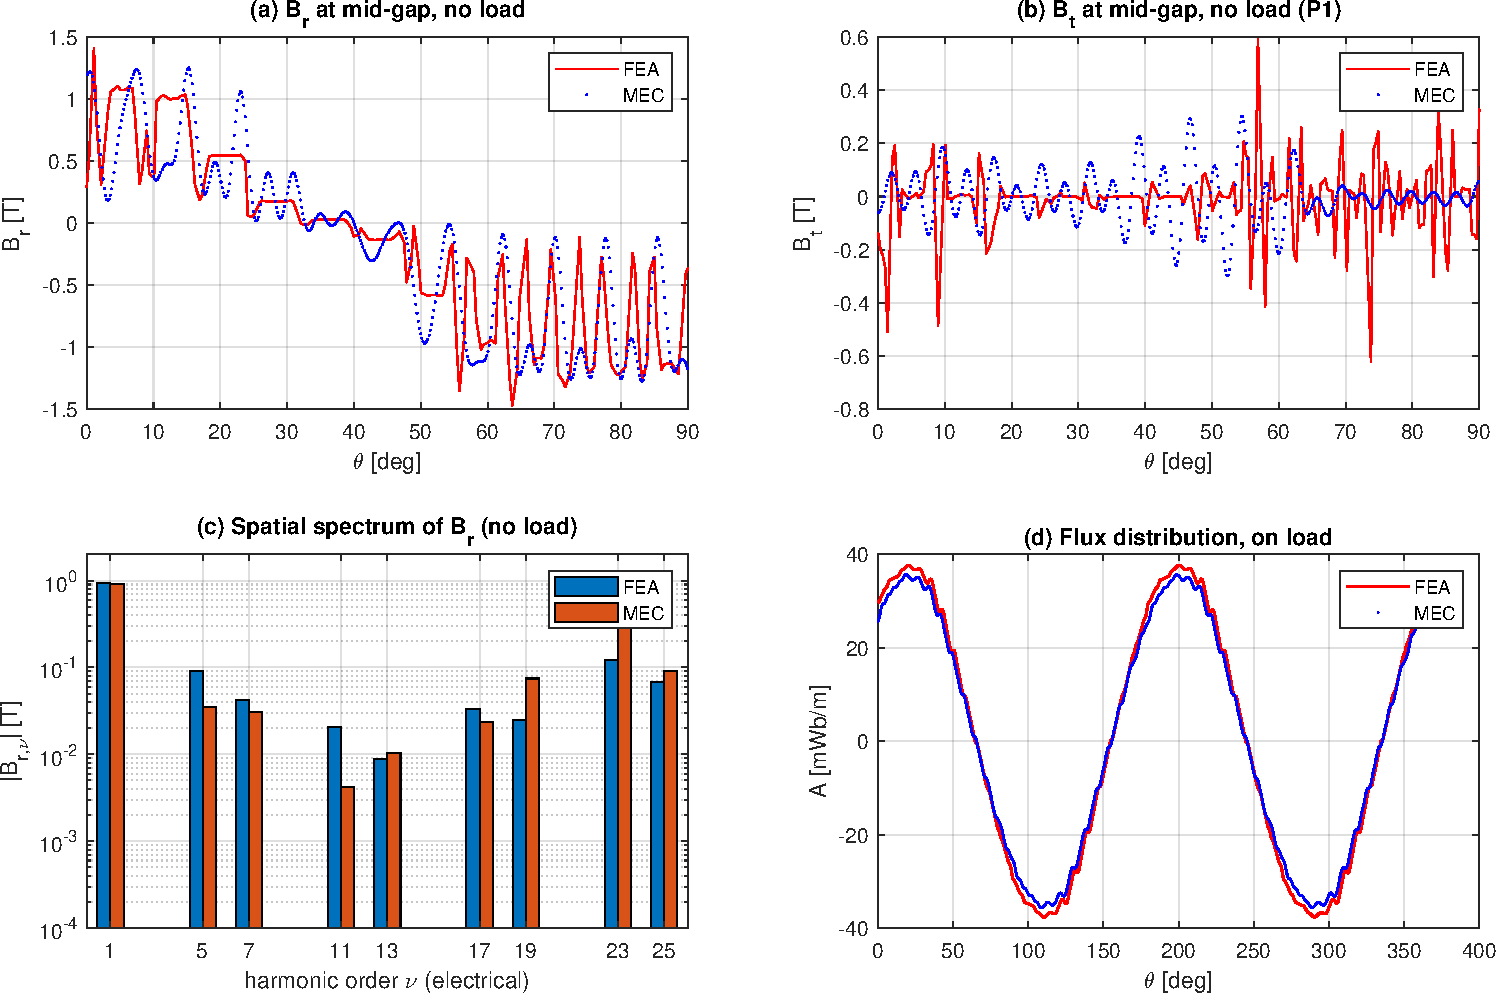
\includegraphics[width=\textwidth,height=0.44\textheight,keepaspectratio]{article_IV_champs.pdf}
\caption{Induction machine, \SI{18.5}{\kilo\watt}, network against
two-dimensional finite elements. \textbf{(a)} Radial flux density at
mid-gap, no load. \textbf{(b)} Tangential component at the same point,
in the conforming basis. \textbf{(c)} Spatial spectrum of the radial
component, on which the fundamental and the slot orders are separated.
\textbf{(d)} Flux distribution on load, where the saturation of the
teeth becomes visible.}
\label{fig:im_field}
\end{figure*}

\paragraph{What the fundamental does not say.}
A fundamental within \SI{0.3}{\percent} constrains one number out of a
whole waveform, and a figure showing two curves does not say how far
apart they are. Table~\ref{tab:fielderr} supplies the three indicators
that were missing: a pointwise root-mean-square deviation, a maximum
pointwise deviation, and the spatial spectrum of $B_r$ tabulated against
the reference. The network field is evaluated \emph{at the angles of the
finite-element sampling itself}, so the difference is pointwise and
exact rather than interpolated, and the two waveforms are registered on
the phase of the fundamental, no offset is fitted. The registration is
carried out on the operator's own harmonic amplitudes instead of on a
sampled estimate, because the condensed operator carries content up to
$n=\num{8192}$, which aliases onto the fundamental bin of a
\num{1000}-point grid; the two estimators are then checked against each
other and agree to better than \SI{5e-5}{\radian}.

The answer is unfavourable and is reported as such. Taking first the
network's own rotor position, $\varphi=0$, which is the one every other
result in this paper uses: at no load the root-mean-square deviation of
$B_r$ is \SI{0.406}{\tesla}, or
\SI{56.3}{\percent} of the root-mean-square of the reference, and the
largest pointwise deviation is \SI{1.36}{\tesla}, \SI{92.7}{\percent} of
the reference peak. The tangential component, the one a network of
radial branches cannot produce at all, and which this closure produces
to within \SI{6.1}{\percent} in root-mean-square, deviates pointwise by
\SI{130.2}{\percent} of the reference's own root-mean-square.
\emph{A fundamental accurate to
three parts in a thousand coexists with a waveform that is wrong almost
everywhere.} That is not a paradox: it is the distinction this paper
draws throughout between a quantity obtained by integration and a
quantity read at a point, and it is stated here with numbers rather than
asserted.

\paragraph{A second degree of freedom, and it is not free.}
Registering on the fundamental fixes the angular origin on the
\emph{stator} side and nothing else. The comparison carries a second
parameter that neither side declares: the mechanical position
$\varphi$ of the rotor. The network fixes it at $\varphi=0$, the
reference snapshot does not state its own, and no single rigid rotation
can register the stator-borne family of orders $kN_{\mathrm{s}}\pm p$
and the rotor-borne family $kN_{\mathrm{r}}\pm p$ at once.

That parameter is identifiable, and identifying it is not fitting the
model: it recovers an initial condition of the \emph{reference} that the
reference does not report. Rebuilding the operator at each position and
sweeping $\varphi$ over one rotor slot pitch, the exact period, verified
rather than assumed, gives a single isolated minimum in each condition,
at \SI{0.976}{\degree} mechanical at no load and \SI{1.236}{\degree} on
load, against a rotor slot pitch of \SI{8.182}{\degree}. The second
local minimum is higher by \SI{54}{\percent} and \SI{11}{\percent}
respectively, so the position is determined and not merely fitted.

\emph{The result is unfavourable, and it bears on the four field figures
above rather than only on the waveform.} Matching the rotor position
lowers the pointwise deviation of $B_r$ from \SI{56.3}{\percent} to
\SI{37.8}{\percent} at no load and from \SI{90.5}{\percent} to
\SI{75.2}{\percent} on load, and the largest pointwise deviation at no
load from \SI{92.7}{\percent} of the reference peak to
\SI{66.7}{\percent}. But it also moves three of the four agreements
quoted at the head of this section, and moves them the wrong way: the
on-load fundamental from \SI{-2.4}{\percent} to \SI{-4.0}{\percent}, the
no-load tangential root-mean-square from \SI{-6.1}{\percent} to
\SI{-10.0}{\percent}, and the on-load tangential from
\SI{-9.3}{\percent} to \SI{+12.4}{\percent}, a change of sign. Only the
no-load fundamental is stable, \SI{+0.3}{\percent} against
\SI{+0.2}{\percent}.

The reason is in the last column of Table~\ref{tab:fielderr}(b). Over
one rotor slot pitch the tangential root-mean-square disperses by
\SI{35.8}{\percent} at no load and \SI{44.0}{\percent} on load, and the
on-load fundamental by \SI{5.35}{\percent}. \emph{Three of the four
agreements quoted are smaller than the spread of a parameter the
comparison did not match.} They are therefore reported here with that
spread beside them: at one rotor position they are what they are, and as
measurements of the closure they establish only the no-load fundamental,
whose \SI{0.3}{\percent} still sits inside a \SI{1.06}{\percent} spread.

What the matching does \emph{not} remove is the deviation itself. At the
matched position the error energy is still carried by the two slot
families---\SI{40.7}{\percent} stator and \SI{42.4}{\percent} rotor at no
load, \SI{34.7}{\percent} and \SI{35.4}{\percent} on load, and the
fundamental still carries none of it. The residual is a property of the
closure, not of the registration.

Where the deviation lives is more informative than its size. Decomposing
the error energy by spatial order, exactly, by Parseval, the
reconstruction agreeing with the pointwise mean square to \num{3e-15}
relative, the fundamental carries \SI{0.0}{\percent} of it at no load.
Orders anchored on the stator slotting, $kN_s\pm p$, carry
\SI{41.9}{\percent}; orders anchored on the rotor slotting, $kN_r\pm p$,
carry \SI{46.6}{\percent}; the two orders common to both families carry
\SI{4.4}{\percent}, and the remaining \num{459} orders carry
\SI{7.2}{\percent} between them. The deviation is therefore not a
diffuse modelling error but a misestimate of two slot-harmonic
families, the sidebands the operator exists to resolve. That both
families are implicated is what makes the next paragraph necessary: one
of the two is anchored on a part of the geometry whose position the
comparison had not matched.

One expectation is not borne out, and it survives the matching. If the
residual were governed by the regions where the surface grid is
coarsest, the deviation would concentrate under the slot openings. It
does not. At the matched rotor position the stator openings carry
\SI{16.2}{\percent} of the no-load error energy on \SI{19.2}{\percent}
of the reference sampling points, and the rotor openings
\SI{15.7}{\percent} on \SI{17.2}{\percent}, both slightly \emph{less}
than their share of the circumference. The waveform
deviation is distributed, not localised beneath the openings. This does
not overturn the diagnosis of Section~\ref{sub:im_tests}, which concerns
saturation in the rotor iron rather than the field in the gap, but it
removes one form of support for it.


The local probes of the refined mesh are reported with a reservation
that must be read before the numbers, because it concerns their
provenance rather than their value. \emph{They do not come from the
chain that produces every other result in this paper.} The performance
network condenses the operator in the hat basis at $N_h=\num{8192}$; the
probe chain calls a separate air-gap routine which imposes the
piecewise-constant basis and truncates at $N_h=100$, a ratio of 82. The
consequence is measurable: sweeping the probe truncation over a factor
of eight moves the readings by up to \SI{5.55}{\percent}, the worst
being the rotor tooth, the very region the preceding section named as
the most likely site of the residual error. Refinement does not close
the gap to the reference either, the stator tooth standing at
\SI{+20.6}{\percent} at $N_h=100$ and \SI{+18.9}{\percent} at
$N_h=800$. The eight reference values are themselves maxima read from
field maps instead of exported quantities, so they are not
re-derivable.

These probes are therefore reported as an indication of regional
saturation level and not as a validated output. The rotor tooth reaches
\SI{2.03}{\tesla} in the network against \SI{1.93}{\tesla} in the
reference; that the model runs high in precisely the region where its
surface grid is coarsest is consistent with the diagnosis of
Section~\ref{sub:im_tests} and is the reason a rotor-side tiling
refinement is proposed rather than a change of closure.

\subsection{Absence of Measurement, and the Test That Would Settle the Claim}
\label{sub:measurement}

\emph{No measurement is presented in this paper and none is claimed.}
The comparison throughout is against a two-dimensional finite-element
field solution; the claim that Carter's factor is low in this regime is
therefore a claim against a numerical reference, not against a machine.
The claim concerns a coefficient that machine designers use and that is
directly measurable, which is why the experiment below is worth
specifying.

The decisive experiment is standard and inexpensive. A \emph{no-load
magnetising test} at several supply voltages, with the machine at
synchronous speed or uncoupled, yields the magnetising reactance as a
function of flux level; extrapolating to zero saturation gives $X_{m0}$,
which is exactly the quantity of \eqref{eq:kcdef}. Because the two
closures differ by twenty percentage points on the no-load
current---\SI{+1.5}{\percent} for Carter against \SI{+21.6}{\percent}
for the converged operator, Table~\ref{tab:price}, a measurement of
ordinary laboratory accuracy separates them decisively. It does not
require a precision bench.

The accuracy that suffices, stated so that the test can be specified
rather than merely invoked: \SI{\pm0.5}{\percent} on line current and on
line voltage; stator resistance measured four-wire at a
\emph{recorded} winding temperature; and at least four voltage points
spanning the saturating region, so that the extrapolation to zero
saturation is itself supported instead of assumed. At that class the
measurement resolves a twenty-point difference by a wide margin, and
would also bound the residual of Section~\ref{sub:im_tests}, which the
present work can only locate.

\begin{table*}[tp]
\centering
\begin{threeparttable}
\footnotesize
\begin{tabular}{@{}llrrrrr@{}}
\toprule
\multicolumn{7}{@{}l}{\emph{(a) pointwise deviation of the waveform}}\\
\midrule
& & reference & \multicolumn{2}{c}{at $\varphi=0$} & \multicolumn{2}{c}{matched\tnote{a}}\\
\cmidrule(lr){3-3}\cmidrule(lr){4-5}\cmidrule(lr){6-7}
condition & comp. & rms (\si{\tesla}) & rms (\si{\tesla}) & of rms & rms (\si{\tesla}) & of rms\\
\midrule
no load & $B_r$ & \num{0.7207} & \num{0.4055} & \SI{56.3}{\percent} & \num{0.2725} & \SI{37.8}{\percent}\\
no load & $B_t$ & \num{0.1282} & \num{0.1669} & \SI{130.2}{\percent} & \num{0.1520} & \SI{118.5}{\percent}\\
on load & $B_r$ & \num{0.7457} & \num{0.6748} & \SI{90.5}{\percent} & \num{0.5606} & \SI{75.2}{\percent}\\
on load & $B_t$ & \num{0.1309} & \num{0.1744} & \SI{133.2}{\percent} & \num{0.2003} & \SI{153.0}{\percent}\\
\midrule
\multicolumn{7}{@{}l}{\emph{(b) the four field figures of this section,
against the rotor position}}\\
\midrule
& & reference & \multicolumn{2}{c}{deviation} & \multicolumn{2}{c}{spread\tnote{b}}\\
\cmidrule(lr){3-3}\cmidrule(lr){4-5}\cmidrule(lr){6-7}
condition & quantity & (\si{\tesla}) & at $\varphi=0$ & matched & \multicolumn{2}{c}{over one pitch}\\
\midrule
no load & $B_{g1}$ & \num{0.942} & \SI{+0.3}{\percent} & \SI{+0.2}{\percent} & \multicolumn{2}{c}{\SI{1.06}{\percent}}\\
no load & $B_t$ rms & \num{0.128} & \SI{-6.1}{\percent} & \SI{-10.0}{\percent} & \multicolumn{2}{c}{\SI{35.8}{\percent}}\\
on load & $B_{g1}$ & \num{0.920} & \SI{-2.4}{\percent} & \SI{-4.0}{\percent} & \multicolumn{2}{c}{\SI{5.35}{\percent}}\\
on load & $B_t$ rms & \num{0.131} & \SI{-9.3}{\percent} & \SI{+12.4}{\percent} & \multicolumn{2}{c}{\SI{44.0}{\percent}}\\
\midrule
\multicolumn{7}{@{}l}{\emph{(c) spatial spectrum of $B_r$ at mid-gap
(\si{\tesla}), at $\varphi=0$}}\\
\midrule
& & \multicolumn{2}{c}{no load} & \multicolumn{2}{c}{on load} & \\
\cmidrule(lr){3-4}\cmidrule(lr){5-6}
$\nu$ & & network & reference & network & reference & \\
\midrule
1  & & \num{0.945211} & \num{0.941900} & \num{0.898254} & \num{0.919739} & \\
5  & & \num{0.075866} & \num{0.090168} & \num{0.093052} & \num{0.049075} & \\
7  & & \num{0.009612} & \num{0.042086} & \num{0.041872} & \num{0.018762} & \\
11 & & \num{0.006766} & \num{0.020466} & \num{0.044336} & \num{0.047561} & \\
13 & & \num{0.025158} & \num{0.008786} & \num{0.037186} & \num{0.036361} & \\
17 & & \num{0.055003} & \num{0.033296} & \num{0.031170} & \num{0.023234} & \\
19 & & \num{0.015394} & \num{0.024553} & \num{0.134026} & \num{0.074595} & \\
23 & & \num{0.065611} & \num{0.122679} & \num{0.531300} & \num{0.290147} & \\
25 & & \num{0.195637} & \num{0.068755} & \num{0.145853} & \num{0.190115} & \\
\bottomrule
\end{tabular}
\begin{tablenotes}[flushleft]\footnotesize
\item[a] At the rotor position identified for each reference snapshot by
minimising the deviation over one rotor slot pitch:
\SI{0.976}{\degree} mechanical at no load, \SI{1.236}{\degree} on load,
against a pitch of \SI{8.182}{\degree}. This recovers an initial
condition of the reference, which the reference does not report; it fits
nothing in the model. The minimum is isolated in both conditions, the
next local minimum is higher by \SI{54}{\percent} and
\SI{11}{\percent}, and the sweep period was verified, not assumed.
\item[b] Full spread of the quantity as $\varphi$ traverses one rotor
slot pitch. Where this exceeds the deviation beside it, the figure
measures the choice of rotor position more than it measures the closure.
That is the case for three rows of four.
\item Chain of Section~\ref{sub:im_fields}: condensed operator at tiling
$(17,4)$, $N_h=\num{8192}$, hat basis, rebuilt at each rotor position.
At $\varphi=0$ the four field figures quoted in
the text above are reproduced to better than \num{1e-4} absolute, which
is the check that the chain measured here is the one the paper reports.
Network amplitudes are the operator's own harmonic amplitudes, not read
from a sampled waveform.
\end{tablenotes}
\end{threeparttable}
\caption{\emph{(a)} Waveform deviation of the mid-gap field against
two-dimensional finite elements, evaluated pointwise at the reference
sampling angles and registered on the fundamental phase, at the
network's rotor position and at the reference's own; \emph{(b)} what the
unmatched rotor position was worth on the four figures this section
quotes; \emph{(c)} the spatial spectrum behind the deviation. A
fundamental within \SI{0.3}{\percent} coexists with a waveform deviation
above half the reference root-mean-square.}
\label{tab:fielderr}
\end{table*}


%======================================================================

\section{Accuracy Trade-Off and Its Diagnosis}
\label{sec:price}

The converged closure is not free. Table~\ref{tab:price} places the
three air-gap models side by side against the finite-element reference:
Carter's factor, the piecewise-constant operator as previously
published, and the converged hat-basis operator of
Section~\ref{sec:p1}.

The magnetising branch pays. The no-load current rises from
\SI{9.921}{\ampere} to \SI{10.323}{\ampere}, that is
\SI{+21.6}{\percent} above the reference instead of
\SI{+16.9}{\percent}, and the saturated magnetising reactance falls to
\SI{-10.6}{\percent} instead of \SI{-6.4}{\percent}. Everything else
moves very little: the air-gap electromotive force by
\SI{-0.22}{\percent} and the rated torque by \SI{-0.40}{\percent}
relative to the published values.


\subsection{Quantities Improved by the Piecewise-Linear Basis}

Reporting only Table~\ref{tab:price} would misdescribe the change, and
the formulation matters here. \emph{The hat basis concentrates the error
on the magnetising branch and improves everything that depends on it
weakly.} Table~\ref{tab:balance} gives the three quantities that move.

\begin{table}[!ht]
\centering
\begin{threeparttable}
\footnotesize
\begin{tabular}{lrr}
\toprule
quantity & piecewise constant & hat \\
\midrule
$B_t$ rms on load (tooth path)    & $-15.98\%$ & $\bm{-9.32\%}$\\
$B_{g1}$ at no load               & $+0.18\%$  & $+0.34\%$\\
$B_{g1}$ on load                  & $-2.91\%$  & $\bm{-2.36\%}$\\
\bottomrule
\end{tabular}
\begin{tablenotes}[flushleft]\footnotesize
\item The hat
column reproduces the corresponding run record to \SI{0.003}{\percent}; the
piecewise-constant column is at $n_T=6$, $n_O=2$, $N_h=\num{3088}$, the
configuration in which $X_{m0}=\SI{64.781}{\ohm}$ was published.
\end{tablenotes}
\end{threeparttable}
\caption{Effect of the hat basis on the field quantities. Both columns
are produced by one execution in the two bases, at the tiling and
truncation each was published with.}
\label{tab:balance}
\end{table}

Two of the three improve, and the direction is the one the diagnosis
predicts. The third does not: the no-load fundamental moves from
\SI{+0.18}{\percent} to \SI{+0.34}{\percent}, a degradation of
\num{0.16} point on a quantity whose spread over one rotor slot pitch is
\SI{1.06}{\percent} (Table~\ref{tab:fielderr}b) and which this
comparison therefore does not resolve. The quantities that improve are those the
magnetising branch governs least: the tangential field, carried by the
tooth-to-tooth path rather than by $X_m$, and the fundamental air-gap
flux density, which the operator fixes from the geometry.

Two of these three rows are new, and they replace values that could not
be reproduced. An earlier version of this work reported the on-load
tangential field at \SI{-12.6}{\percent} in the piecewise-constant basis
and the on-load fundamental at \SI{-1.2}{\percent}, and drew from the
second the conclusion that the hat basis degraded one quantity. Neither
figure survives regeneration: both came from a table rather than from an
execution, and computed in the configuration in which they were
published they read \SI{-15.98}{\percent} and \SI{-2.91}{\percent}.
\emph{The hat basis improves that row too.} The claim that it degrades a
field quantity is withdrawn; what it costs is stated in
Table~\ref{tab:price} and is confined to the magnetising branch.

\subsection{Existence, Not Accuracy, as the Argument for the Hat Basis}

The table above is not a claim of improved accuracy, and it would be
weak if it were: on the headline quantity the converged model is further
from the reference than the one it replaces. The argument is different,
and it is sufficient.

Appendix~\ref{app:trace} proves in closed form that in the
piecewise-constant basis the energy series \emph{diverges}. The
\SI{64.78}{\ohm} previously reported is therefore not a value of
$X_{m0}$; it is one point on a curve that has no limit. \emph{A number
that changes with the truncation is not a prediction, even when it falls
closer to the reference.}

What the hat basis buys is that $X_{m0}$ exists. The price of that
existence is \num{4.7} points on the no-load current
deviation---\SI{+16.87}{\percent} against \SI{+21.61}{\percent}, and
it is visible, bounded and stated.

\subsection{Absence of a Dominant Model and the Need for an Explicit Choice}

A referee will observe what Table~\ref{tab:price} shows plainly: Carter
is the \emph{best} of the three on the no-load current
(\SI{+1.5}{\percent}) and the \emph{worst} on the saturated magnetising
reactance (\SI{+9.7}{\percent}); the converged operator is the reverse.
No model dominates on every line.

\emph{What the closure is, and is not, usable for.} Answering ``is this
well posed?'' does not answer ``should a designer use it?'', and the
second question deserves a bounded answer on the paper's own evidence.
The operator is usable for the \emph{tangential} field and the
slot-harmonic content, which a permeance closure does not approximate
badly but does not produce at all; for the saturated magnetising
reactance, where it is closer than Carter; and for the fundamental
air-gap flux density. It is \emph{not} usable, as it stands, for
magnetising-current or power-factor prediction: \SI{+21.6}{\percent} on
$I_0$ is a design-relevant error and it is not explained, only located
(Section~\ref{sub:im_tests}). And the corrected slotting ratio is
unsaturated, so it cannot be substituted into a classical saturated
design chain by rescaling $X_m$.

We retain the converged operator, and the reason is not that it wins on
count. Carter's agreement on $I_0$ is obtained from a formula whose
hypotheses this geometry violates, see \eqref{eq:b0g}, and it comes
with no way of knowing, from within the model, when it will fail. The
operator has hypotheses that the geometry satisfies, and a truncation
whose effect is bounded and measurable. That is the trade the paper
proposes; it should be judged as such rather than on a row count.

\subsection{Probable Origin of the Residual Error}

The remaining \SI{-6.0}{\percent} on rated torque, the deviation of the
retained hat-basis model, not the \SI{-5.7}{\percent} of the
piecewise-constant column, is not explained here,
but the candidates can at least be ranked, which is more useful than
listing them. \emph{Ranked by the order of magnitude each could
plausibly carry}: the rotor-slot-opening representation in the tiling,
which the probe evidence below points to and which is the only candidate
of the right size; the harmonic cage and end-ring model, which
Section~\ref{sub:standstill} shows dominates at standstill but whose
rated-point contribution is bounded by the \SI{+0.57}{\percent} skew
residue and the \SI{16.7}{\percent} share of $R'_r$; the winding
temperature, worth a few tenths of a percent on the copper loss and
nothing on the torque; and the tiling non-convergence, which
Section~\ref{sub:im_coupled} measures at \SI{0.275}{\percent} on the
torque and therefore \emph{excludes} as the principal cause. The first
is the only one of the four that can carry six points, and the evidence
points in its direction. The rotor tooth carries the
highest flux density of the machine, and it is also the region where the
model is least converged: the local probes of
Section~\ref{sub:im_fields} drift by \SI{5.55}{\percent} under
refinement of the surface truncation, and the rotor tooth is the worst
of the eight. A rotor-side tiling refinement is therefore the first
thing to try, and it is a development rather than an adjustment, which
is why it is stated as a lead and not as a result.

A fifth candidate exists and is deliberately left out of that ranking.
The surface basis does not represent the constant function exactly on the
tiled grid (Section~\ref{sub:hatdefect}), and the bias that follows is
measured on the homopolar mode alone. Ranking it would require knowing
what it does to the orders $n\ge1$ that carry $X_m$, and that has not
been measured. It is named here so that the four ranked candidates are
not read as an exhaustive list.

%=======================================================================
\section{Torque Ripple: a Capability of the Closure, Outside the Audited Chain}
\label{sec:skew}

Because the operator delivers both field components on the bore, the
Maxwell-stress torque is available at every rotor position without a
co-energy derivative, and a ripple map $\Delta T(\theta)$ can be built
and injected into the mechanical equation. Nineteen field solutions over
two slot pitches suffice. This is a capability of the closure rather
than of the network: a set of radial branches produces no tangential
flux density at all, so no ripple map can be formed from it.

\subsection{Elements Not Inherited from Section~\ref{sec:p1}}
\label{sub:ripple_scope}

One point of routing must be settled before any figure is quoted,
because it decides what the results of this section are evidence for.

The ripple map is not built from the condensed tooth operator of
Section~\ref{sec:twosurface}. It is built from the air-gap treatment
internal to the refined mesh, which resolves the annulus with its own
cells rather than through the surface admittance matrix. The map
therefore never passes through the projection whose conformity
Section~\ref{sec:p1} establishes, and \emph{the convergence result
proved there does not extend to it}. The consequence should be stated
once, plainly, and carried to the conclusion: \emph{this section
contributes no evidence for or against the central claim of the paper}.
What it demonstrates is that a ripple map \emph{exists at all}, because
the closure delivers a tangential field; that is a capability, not a
validation.

This has a measurable consequence, and it is the reason the point is
raised rather than left implicit. Exchanging the surface basis at
constant chain moves the on-load ripple by \SI{-0.38}{\percent}. In a
paper whose central claim is that the choice of surface basis decides
whether the condensed operator has a limit at all, a quantity that
barely notices that choice would be read as evidence of robustness. It
is not. The insensitivity follows from the routing: what is not
projected onto the basis cannot depend on it. Reporting it as
robustness would attribute to the formulation a property it does not
have here.

Two consequences for how the figures below should be read. The ripple is
not covered by the convergence argument and is reported as a
capability, the closure delivers a tangential field, so a
Maxwell-stress map exists at all, not as a converged prediction. And
because the map lies outside the audited chain, its provenance is named
explicitly: every ripple figure in this section is produced by the
single chain declared for that quantity in the reproducibility
statement, and by no other. A second implementation available to the
authors returns \SI{128}{\newton\metre} for the same quantity. That discrepancy
is not explained, is not attributable to the surface basis, and is under
investigation; until it is resolved, the second value is not quoted and
the first is not presented as converged.

\subsection{Validity of the Ripple Map Under Load}

Fig.~\ref{fig:im_ripple} shows the on-load run-up in five panels:
panel~(a) the speed, panel~(b) the torque with its ripple superimposed,
panel~(c) the stator current, panel~(d) a magnification of the torque
over a few slot pitches, which is the panel the ripple figure is read
from, and panel~(e) the dynamic trajectory in the torque--speed plane.
The quantity discussed below is the peak-to-peak value of panel~(d);
the four others are shown so that it can be seen to belong to a run
that is otherwise correct. The single-slice ripple is
\SI{108.2}{\newton\metre} peak-to-peak against \SI{105.5}{\newton\metre}
in the reference, that is \SI{+2.6}{\percent}. \emph{That agreement must
be read beside the implementation spread declared above}: a second
implementation of the same quantity returns \SI{128}{\newton\metre},
\SI{18}{\percent} away, so the comparison is narrower than the
reproducibility of the quantity it compares and is reported as a
capability rather than as an agreement. The run-up reaches \SI{95}{\percent} of synchronous
speed in \SI{0.141}{\second} against \SI{0.122}{\second}, and the mean
speed and torque of the settled regime are reproduced within
\SI{0.1}{\percent} and \SI{0.7}{\percent}.

\begin{figure*}[!tb]
\centering
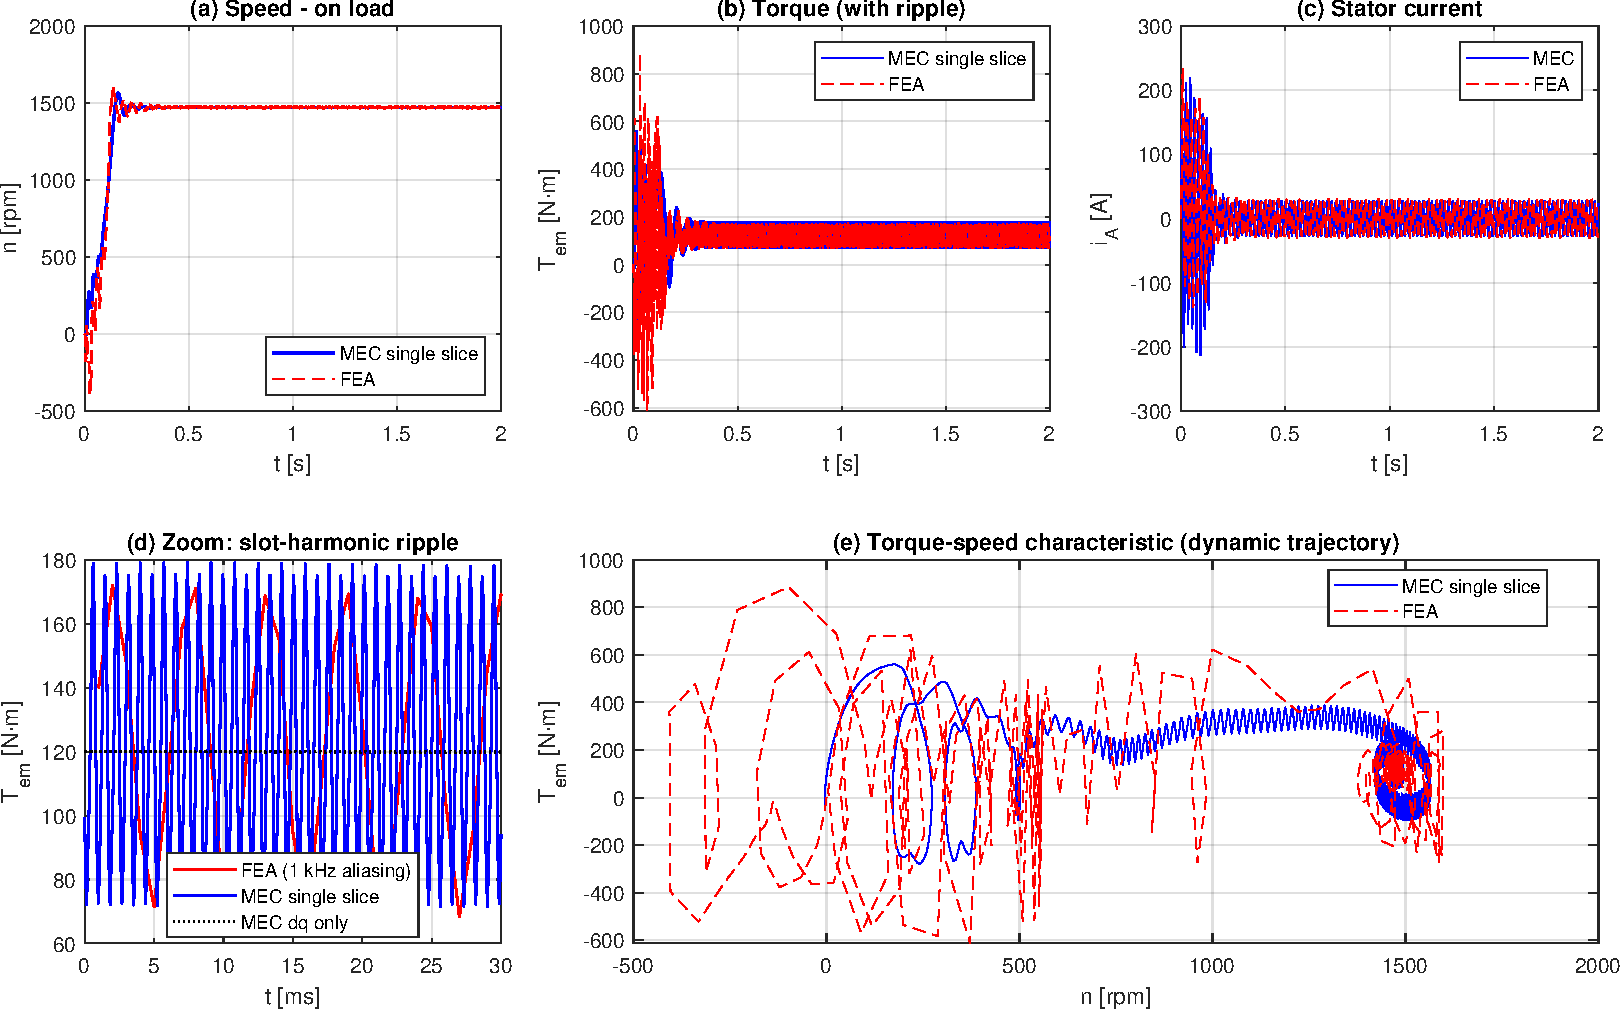
\includegraphics[width=\textwidth,height=0.44\textheight,keepaspectratio]{article_V_1tranche_en_charge.pdf}
\caption{Induction machine on load. \textbf{(a)} Speed.
\textbf{(b)} Torque with its slot-harmonic ripple superimposed.
\textbf{(c)} Stator current. \textbf{(d)} A
\SI{30}{\milli\second} window of the settled ripple, which is the panel
the ripple figure is read from. \textbf{(e)} Dynamic torque--speed
trajectory. The ripple map is
built from nineteen Maxwell-stress evaluations and injected into the
mechanical equation. Both models are single-slice.}
\label{fig:im_ripple}
\end{figure*}

\subsection{Loss of Validity at No Load and Its Probable Cause}

At no load the model returns \SI{79.5}{\newton\metre} against
\SI{10.3}{\newton\metre}: a factor of eight.
Fig.~\ref{fig:im_ripple_nl} repeats at no load the arrangement of
Fig.~\ref{fig:im_ripple}, panel for panel, so that the two operating
points are compared directly rather than through two differently drawn
figures: panel~(a) the speed, panel~(b) the torque with its ripple
superimposed, panel~(c) the stator current, panel~(d) the magnified
torque over a few slot pitches, and panel~(e) the trajectory in the
torque--speed plane. Panels~(a), (b), (c) and~(e) are unremarkable: the
no-load run is correct in every respect a run can be correct in. The
failure is confined to panel~(d), and that confinement is itself the
evidence for what follows. The cause is not in the closure. The
field bench computes the ripple from a magnetostatic sequence in which
the cage currents are held at their steady-state value, so the damping
of the slot-harmonic field by the bar currents it induces is absent. On
load the fundamental cage current dominates and the omission is hidden;
at no load nothing masks it.

\begin{figure*}[!tb]
\centering
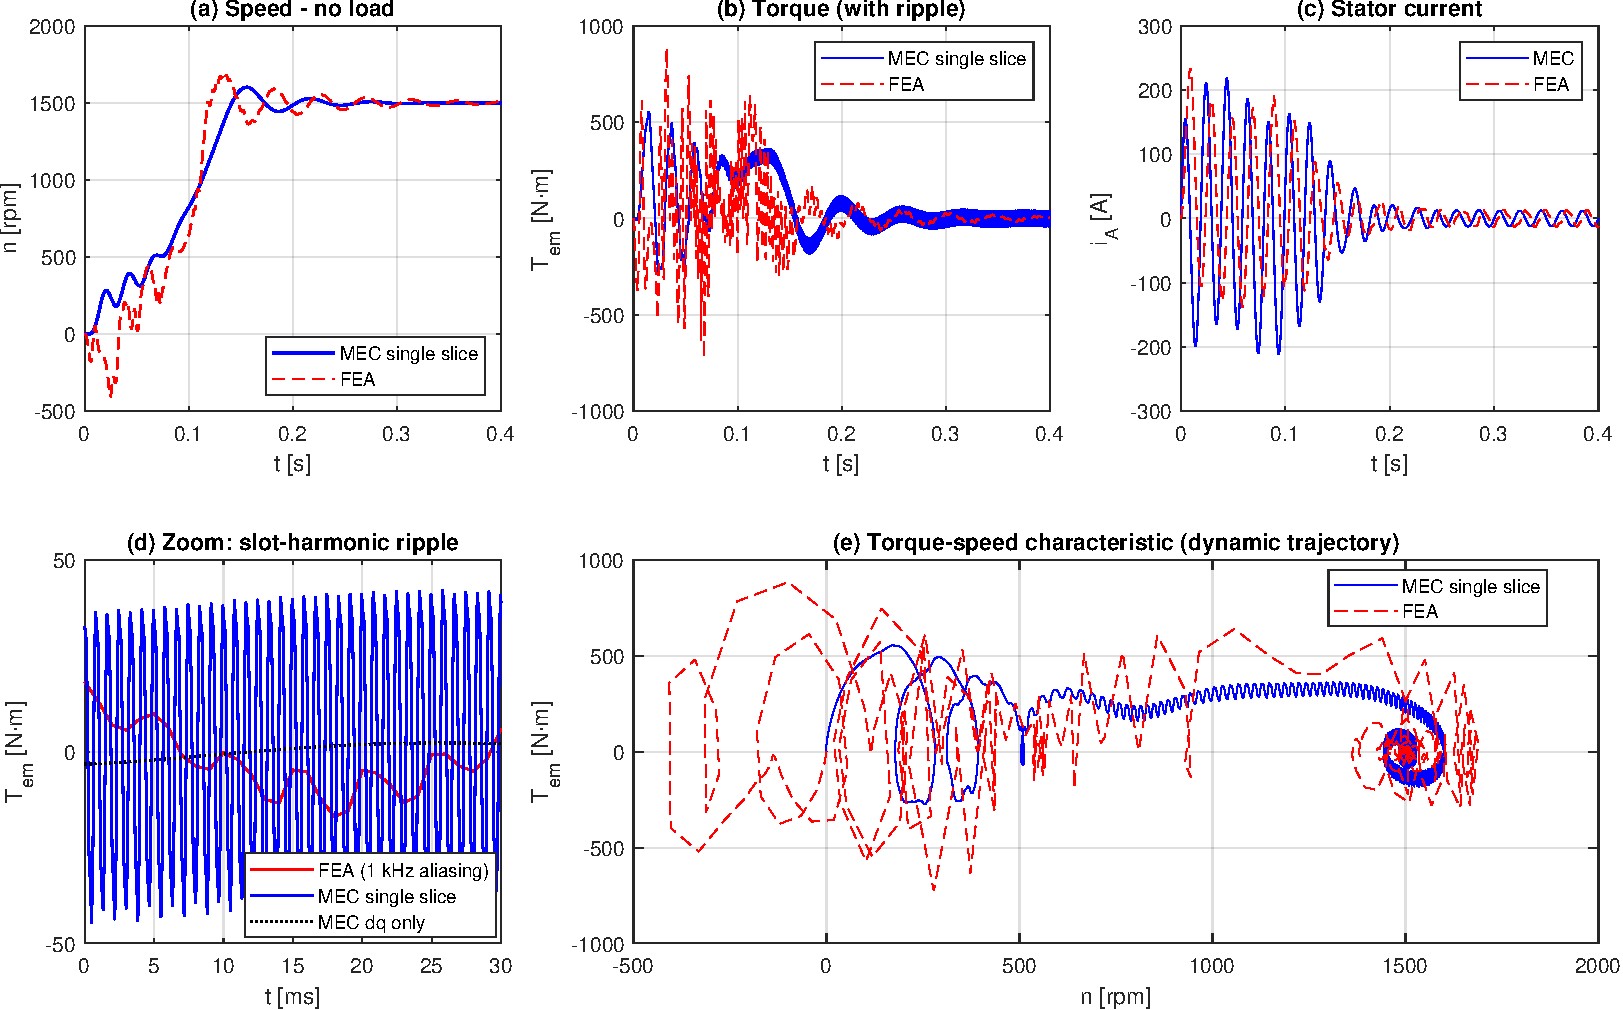
\includegraphics[width=\textwidth,height=0.44\textheight,keepaspectratio]{article_V_1tranche_a_vide.pdf}
\caption{The same construction at no load, panel for panel with
Fig.~\ref{fig:im_ripple}, where it fails by a factor of eight.
\textbf{(a)} Speed. \textbf{(b)} Torque with ripple. \textbf{(c)}
Stator current. \textbf{(d)} Settled ripple, the only panel in which
the failure appears. \textbf{(e)} Torque--speed trajectory. The cage currents of the field bench are frozen at their
steady-state value, so the slot-harmonic field is not damped by the bar
currents it induces; on load the fundamental cage current hides this,
at no load nothing does.}
\label{fig:im_ripple_nl}
\end{figure*}

The ripple map is therefore valid on load and must not be used at no
load without a harmonic cage model. We report the no-load figure rather
than omitting it, because the ratio of eight is what makes the
limitation legible: a reader who saw only the on-load agreement would
have no way of knowing where the map stops being usable.

\subsection{The Skew Caveat and Its Non-Applicability to This Result}

Both models are evaluated on a single slice, so the attenuation of the
ripple by skew is absent from both and does not enter the
comparison~\cite{gyselinck}. That statement appeared in an earlier
version of this work, and it is true, but it was true for a reason that
had not been checked, and the reason is worth giving because the same
sentence would be false if applied one section earlier.

On the reference side the position is unambiguous. The project sets
\texttt{UseSkewModel} true with an angle of \ang{7.5}, but
\texttt{NumberOfSlices} equal to one, in each of its four setups. A
single slice admits no relative rotation, hence no axial averaging: the
field solution is that of a straight cross-section.

On the network side the position is not symmetric, and this is the point
that matters. The network applies a skew reduction factor to every space
harmonic of the cage impedance, and Section~\ref{sub:im_scope} disables
it precisely so that the equivalent circuit is comparable with an
unskewed reference. \emph{The ripple map does not inherit that problem},
because it does not pass through the harmonic cage branches at all: the
bar currents injected into the field solution are a pure fundamental
spatial distribution, $i_b(\theta_k)=\sqrt{2}\,I_b\cos(p\theta_k-\psi_2)$,
imposed from the equivalent circuit rather than solved harmonic by
harmonic. The harmonic skew factor, which moves the standstill torque by
\SI{16}{\percent} (Section~\ref{sub:standstill}), leaves this figure
untouched. What does reach it is the \emph{fundamental} factor
$k_{sq}=\num{0.997147}$, through the amplitude of the imposed currents,
and its effect on the quantities that set those amplitudes is between
\SI{0.1}{\percent} and \SI{0.4}{\percent}.

Two consequences follow, and they point in opposite directions. The
comparison of this section is sound as it stands. But the ripple it
compares is that of a machine whose cage responds only at the
fundamental, and the reference, being a genuine field solution, lets
the slot-harmonic currents flow. That is the same omission identified at
no load, seen from the other side, and it is the reason the on-load
agreement should be read as a validation of the \emph{torque
functional} rather than of the ripple amplitude itself.



%======================================================================

\section{Conclusion}
\label{sec:conclusion}

An annulus bounded by two slotted iron surfaces can be closed exactly.
The Dirichlet-to-Neumann operator of that annulus, assembled on a tiling
in which tooth faces and slot openings pave the bore, and condensed onto
the tooth nodes of a reluctance network by a Schur complement, becomes
an ordinary, if dense, network element. The redistribution of flux
beneath the slot opening is solved rather than parameterised, and no
fringing coefficient, effective gap or coupling width enters anywhere.

Applied to an \SI{18.5}{\kilo\watt} cage induction machine, the operator
returns a slotting ratio that exceeds the classical one at every
discretisation computed:
\begin{equation*}
k_{\mathrm{C}}\in[\num{1.2978},\,\num{1.3889}]
\qquad\text{against}\qquad
k_{\mathrm{C}}^{\text{Carter}}=\num{1.2665},
\end{equation*}
that is \SI{+2.5}{\percent} to \SI{+9.7}{\percent} over nine tilings,
with no fitted coefficient anywhere in the chain. The excess is expected
in this regime rather than surprising:
Carter's construction maps a single isolated slot in an infinite
half-plane, and here the slot opening is \num{8.23} times the gap while
\emph{both} surfaces are slotted. What is new is that the excess is
measured. A century-old correction, applied daily in machine design, is
\emph{bounded} against a solution that makes none of its assumptions.
The bound is one-sided and it is the result: nine independent
discretisations all exceed the classical value, which falsifies it in
this regime without requiring a converged replacement. The ratio at the
production tiling, \num{1.3320}, is quoted in \eqref{eq:kc} as the value
at one discretisation and is not offered as that replacement.

Two measurements make that bound one-sided in the direction stated, and
both are reported rather than assumed. The tiling is not closed, so the
finest point is below the limit if a limit exists. And the iron
reluctance is finite in both unsaturated solves and identical between
them, which compresses the ratio towards unity: repeated at infinite
iron permeability the same operator returns \num{1.6026} instead of
\num{1.3320}, \SI{+20.3}{\percent} \eqref{eq:muinf}. The quantity
Carter's factor is defined to be is the second one; \emph{the values
this paper reports are the first}, and the gap between them is measured,
declared, and left for the coefficient's users to arbitrate. In neither
sense does the excess over the classical value disappear---it grows.

Two limits belong with that statement. The ratio is \emph{unsaturated},
formed on $X_{m0}$; Section~\ref{sub:im_tests} shows it cannot be
inserted into a saturated design chain by rescaling $X_m$, because the
scaling that would correct the no-load current would overshoot the
saturated reactance. And the comparison is against a finite-element
field solution, not against a machine: no measurement is presented and
none is claimed.

An earlier version of this work reported that the operator reproduced
Carter's ratio to three decimals and offered that agreement as a
validation. It was not one. The piecewise-constant series has no limit,
the curve crosses the classical value on its way past it, and the
agreement was fixed by where the sum was stopped. Withdrawing it is what
makes the correction reportable.

The price is stated rather than absorbed, and it is not small. The
no-load current, which the closure this operator replaces matched to
\SI{1.5}{\percent} \emph{by construction}, is high by
\SI{21.6}{\percent} once that construction is removed, and the saturated
magnetising reactance is low by \SI{10.6}{\percent}. The error is
displaced onto the magnetising branch and concentrated there: everything
that depends on it weakly improves, including the two field quantities
that an earlier version reported as degraded and which do not survive
regeneration. No model dominates, Carter's factor is the best of the
three on the no-load current and the worst on the saturated
reactance, so the paper states which it retains and why, instead of
counting rows.

The argument for the converged closure is not accuracy. On the headline
quantity the converged model is further from the reference than the one
it replaces. The argument is that $X_{m0}$ \emph{exists}: in the
piecewise-constant basis the energy series diverges, so the previously
reported value is one point on a curve with no limit, and a number that
changes with the truncation is not a prediction even when it falls
closer to the reference. What the hat basis buys is a quantity of the
geometry rather than of the discretisation, and the price of that is
visible, bounded and stated.

That argument survives a defect of the same basis, which this paper
reports rather than repairs. A suite of eight invariants, checks the
operator must satisfy whatever the geometry and the discretisation, and
which therefore use neither the finite-element reference nor any
identified constant, holds on six counts to the level of the
arithmetic, two independent routes to the torque agreeing to
\num{1.22e-14}, and fails on two. The two failures are one defect: the
hat basis represents the constant function exactly on a uniform grid and
not on the tiled one, because tooth-face and opening columns have
different widths by design, and at their junctions the hats leave a gap
or an overlap. On the homopolar mode this costs \SI{0.303}{\percent} on
the annulus permeance, it grows with the truncation instead of falling,
and its remedy, an asymmetric hat whose half-widths are the local
half-steps, keeps the projection in closed form. \emph{Whether it
propagates to the slotting ratio is not measured here and is not
inferred.} What the episode establishes beyond this operator is cheaper
than the defect itself: in a chain where constants are identified against
the reference, agreement with the reference cannot distinguish a correct
model from a calibrated wrong one, and a check that needs no reference
can.

Three further limits are declared, each with the sub-model responsible.

The standstill point is not a test of the closure. At $s=1$ every
harmonic slip reaches unity simultaneously, so the harmonic cage
branches are all at their own standstill and govern the result: the
computed torque moves by \SI{16}{\percent} between two settings of a
skew factor, and the parasitic torque of two slot-harmonic orders
accounts for four fifths of the change. What would make that point
informative is a validated harmonic cage, and in particular an end-ring
model better than the one-dimensional skin-effect representation that
carries \SI{16.7}{\percent} of the referred rotor resistance there.

The single-slice ripple map is valid on load and fails by a factor of
eight at no load, because the field bench that builds it freezes the
cage currents at their steady-state value and therefore omits the
damping of the slot-harmonic field. The same omission, seen from the
other side, is why the on-load agreement validates the torque functional
rather than the ripple amplitude.

The local probes of the refined mesh do not come from the chain that
produces the rest of the paper, a different basis and a truncation
smaller by a factor of 82, and they drift by \SI{5.55}{\percent} under
refinement, worst on the rotor tooth. That they run high in precisely
the region where the surface grid is coarsest is the clearest indication
of where the residual error on the magnetising branch lives, and a
rotor-side tiling refinement is the first computation to try.

Finally, a remark on the reference. A numerical reference is not a
measurement, and this one turned out to carry structure that had to be
established before any agreement could be asserted: two families of
determination for the same quantity, differing in resolution by more
than an order of magnitude at high slip; a torque--slip sweep with two
noisy bands whose local scatter reaches \SI{13}{\percent}; and anchor
values in the reference data file that do not reproduce the runs they
purport to summarise. None of this was visible from the published
tables. It became visible only by regenerating every figure from the
raw exports, and that discipline changed the sign of one reported
deviation and the direction of another. We record it because none of it could have been suspected from the
published tables, and because the discipline that revealed it, regenerating every figure from the raw exports rather than carrying a
number forward, is cheaper than the errors it prevents.

%======================================================================

\appendix

\section{Trace Conformity of the Condensed Operator}
\label{app:trace}

Section~\ref{sec:p1} rests on one property of the surface basis. It is
derived here, so that the argument of that section can be checked
without leaving this paper.

\emph{Declared overlap.} The same property, with a numerical
verification on a permanent-magnet machine and a diagnostic that
distinguishes a logarithmic tail from geometric convergence, is the
subject of a companion manuscript submitted concurrently by the present
authors. It is restated here rather than cited because a result on which
Section~\ref{sec:p1} depends should not require a reader to obtain an
unpublished text, and because the two papers are independent in every
other respect. The overlap is confined to this appendix.

Let the bore potential be represented on a tiling of arcs by a basis
$\chi_k$, and let $W_n(k)$ be the projection of $\chi_k$ onto the
harmonic of order $n$. The self-energy of one surface column is
\begin{equation}
Y(k,k)=\sum_{n\le N}\hat{g}_n\,\bigl|W_n(k)\bigr|^{2},
\label{eq:app_energy}
\end{equation}
where $\hat{g}_n$ is the assembled bore admittance of order $n$. Once
$n\gg 1/\Xg$ the annulus kernel degenerates, $\coth(n\Xg)\to1$, and
$\hat{g}_n$ grows \emph{linearly} in $n$.

\emph{Piecewise-constant basis.} The indicator function of an arc of
width $d$ has
\begin{equation}
W_n=\frac{2}{n\pi}\sin\frac{nd}{2},
\label{eq:app_p0}
\end{equation}
whose modulus decays only as $1/n$. The summand of
\eqref{eq:app_energy} therefore behaves as $n\cdot n^{-2}=n^{-1}$: the
series is harmonic and \emph{diverges}. The discrete operator has no
limit, and the truncation $N$ selects a value rather than approximating
one. This is not a rate of convergence that could be improved by
refinement; it is the absence of a limit, and its origin is that a
function with jumps does not belong to $H^{1/2}(\Gamma)$, the trace
space on which the Steklov--Poincar\'e operator is bounded.

\emph{Hat basis.} The continuous piecewise-linear basis has
\begin{equation}
W_n=\frac{4}{\pi n^{2}d}\,\sin^{2}\frac{nd}{2},
\label{eq:app_p1}
\end{equation}
whose modulus decays as $1/n^{2}$. The summand now behaves as
$n\cdot n^{-4}=n^{-3}$, the series converges absolutely, and the
residual tail beyond $N$ decays as $1/N^{2}$. The hat basis lies in
$H^{1/2}(\Gamma)$, which is why the remedy works.

\emph{A diagnostic that needs no limit.} The two cases are told apart by
the increments of the partial sum under successive doublings of $N$.
A harmonic tail contributes $\ln N$, so each doubling adds the same
constant and the ratio of successive increments tends to \emph{one}; a
geometrically convergent series adds a decreasing amount and the ratio
settles \emph{below} one. The ratio is therefore readable from a sweep
alone, without knowing the limit and without assuming one exists, which
is what Section~\ref{sub:kccoincidence} uses.

The whole of Section~\ref{sec:p1} is the transposition of this
statement to the doubly slotted annulus, and Table~\ref{tab:kc} is its
measurement on this machine.

%======================================================================

\section*{Data availability}
The program that generates every figure and table of this paper is
deposited in a public archive under
DOI~\texttt{10.5281/zenodo.XXXXXXX}, together with the dated manifest
that binds each published quantity to the single chain that produced
it.

\bibliographystyle{unsrt}
\bibliography{ArticleII}

\end{document}
